\documentclass[10pt, a4paper]{report}
\usepackage[utf8]{inputenc}
\usepackage{amsfonts}
\usepackage{amsmath}
\usepackage{amssymb}
\usepackage{amsthm}
\usepackage[all,cmtip]{xy}
\usepackage{hyperref}
\usepackage[top=3cm, left=3cm,right=3cm, bottom=3cm]{geometry}
\usepackage{graphicx}
%\usepackage{subfig}
%\usepackage{subfigure}
\usepackage{caption}
\usepackage{subcaption}
\usepackage{float}
\usepackage{tikzsymbols}
\usepackage{algorithm}
\usepackage{mathtools}
\usepackage[noend]{algpseudocode}
\newcommand{\E}[0]{\mathbb{E}}
\newcommand{\N}[0]{\mathbb{N}}
\newcommand{\Ll}[0]{\mathbb{L}}
\newcommand{\R}[0]{\mathbb{R}}
\newcommand{\Pp}[0]{\mathbb{P}}
\newcommand{\p}[0]{\mathfrak{p}}
\newcommand{\I}[0]{\mathcal{I}}
\newcommand{\K}[0]{\mathcal{K}}
\newcommand{\F}[0]{\mathcal{F}}
\newcommand{\Oo}[0]{\mathcal{O}}
\newcommand{\vv}[0]{\mathbf{v}}
\theoremstyle{definition}
\newtheorem{theorem}{Theorem}
\newtheorem{prop}{Proposition}
\newtheorem{lemma}{Lemma}
\newtheorem{coro}{Corollary}
\newtheorem{definition}{Definition}
\newtheorem*{properties*}{Properties}
\theoremstyle{remark}
\newtheorem{rmk}{Remark}
\newtheorem{ex}{Example}






\begin{document}
\begin{titlepage}
	\centering
	
\includegraphics[width=0.6\textwidth]{EPFL-Logo}\par\vspace{1cm}
	%{\scshape\LARGE École polytechnique fédérale de Lausanne \par}
	\vspace{1cm}
	{\scshape\Large Master thesis\par}
	\vspace{1.5cm}
	\hrulefill \\
	{\huge\bfseries A probabilistic approach to the classification of censored functional data \par}
	\hrulefill \\
	\vspace{2cm}
	{\Large William \textsc{Borgeaud dit Avocat}\par}
	\vfill
	{\Large
	supervised by\par
	Prof.~Victor \textsc{Panaretos}}
	
	\vfill
	
	% Bottom of the page
	{\large \today\par}
\end{titlepage}

\tableofcontents

\chapter{Introduction to Functional Data Analysis}
\section{What are functional data?}
We will use the term \textit{functional data} for any data living in some infinite dimensional space. This definition is intentionally vague and encompasses various types of data. By infinite dimensional space, we mean any model of space that does not satisfy some finiteness conditions. For example, infinite dimensional vector spaces or manifolds. Here are some concrete examples of such data and spaces:
\begin{enumerate}
	\item Functions $f:\R \to \R$ \ $\leadsto$ \ $\R^\R$. 
	\item Square integrable measurable functions $f:[0,1] \to \R$ \ $\leadsto$ \ $\L^2[0,1]$.
	\item Continuous closed curves in the plane $f: [0,1] \to \R^2$, $f(0)=f(1)$ \ $\leadsto$ \ $\mathcal{C}(\mathbb{S}^1, \R^2)$.
	\item Amplitudes of square integrable measurable functions $f:[0,1] \to \R$ \ $\leadsto$ \ $\L^2[0,1]/\mathrm{Diffeo}([0,1])$, where $\L^2[0,1] \curvearrowleft \mathrm{Diffeo}([0,1])$ by $f \cdot \gamma = (f\circ \gamma)\sqrt{\frac{d\gamma}{dt}}$.
\end{enumerate}
These four examples show different type of spaces one can study. The first one is a vector space of uncountable dimension. With its standard topology it is not metrizable. The second is a separable Hilbert space with inner product $\langle f,g\rangle = \int_{0}^{1}f(t)g(t)dt$. The third is a separable Banach space with norm $\Vert f \Vert = \max_{z \in \mathbb{S}^1} \Vert f(z)\Vert_{\R^2}$. Finally, the last is a Hilbert manifold, i.e., a separable topological space locally homeomorphic to a Hilbert space.\\
Evidently, some spaces are easier to work with than others. For instance, it is preferable to have a metric to measure the discrepancies between data points. Banach spaces and Hilbert manifold are metrizable, but functions from and to these spaces can be hard to analyze. The extensive theory of operator on Hilbert spaces make them good candidates for functional data analysis, and they are indeed the spaces of choice in most of the literature.\\
In this project, we focus on the separable Hilbert spaces. It is well-known that all such spaces are isomorphic to the space $\ell^2(\R)$ of square summable sequences. However, we will mainly focus on the space $\L^2[0,1]$ as the most common type of functional data are functions depending on time. A famous example of such data is the growth data set from the Berkeley Growth Study, see \cite{growth}. It contains the heights of girls and boys from birth to their 18th year. Graphs of these heigths and their derivative for 5 girls and boys are shown in Figure \ref{fig:growth}.
\begin{figure}[H]
	\centering
	\begin{subfigure}{.5\textwidth}
		\centering
		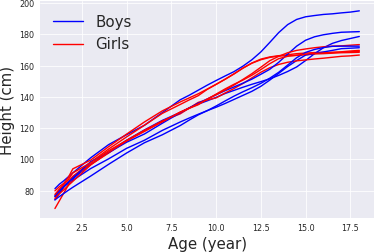
\includegraphics[width=.8\linewidth]{Code/images/11/growth}
		\caption{Height against age}
	\end{subfigure}%
	\begin{subfigure}{.5\textwidth}
		\centering
		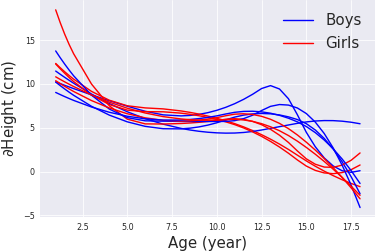
\includegraphics[width=.8\linewidth]{Code/images/11/dgrowth}
		\caption{Derivative of height against age}
	\end{subfigure}
	\caption{}
	\label{fig:growth}
\end{figure}
Questions one may ask on these data are: What are the mean and variance of these curves, and what do these notions mean? Can we classify a given curve as coming from a boy or a girl? How do we deal with the fact that individuals don't have the same ``biological clock''?\\
Functional data analysis deals with this kind of questions. In the next section, we will expose the theory needed to answer the first one.

\section{Stochastic processes on $[0,1]$}
We want to study random functions in $\L^2[0,1]$. There are two possible definitions:
\begin{itemize}
	\item A random function in $L^2[0,1]$ is a random element in $(L^2[0,1],\mathcal{B}(\L^2[0,1]))$, i.e., a measurable map $$X:(\Omega,\mathcal{F},\Pp) \to (L^2[0,1],\mathcal{B}(\L^2[0,1]))$$
	for some probability space $(\Omega,\mathcal{F},\Pp)$.
	\item A random function in $L^2[0,1]$ is a stochastic process on $[0,1]$, i.e., a collection $\{X(t) \mid t\in [0,1] \}$ of random variables defined on a common probability space $(\Omega,\mathcal{F},\Pp)$, such that 
	$$\int_{0}^{1} X^2(t,\omega) dt < \infty \text{ for almost all } \omega.$$ 
\end{itemize}
The first definition is more abstract and somewhat more elegant. However, it is not so practical since, for example, the evaluation at a point is not well-defined in $L^2[0,1]$. On the other hand, it can readily be generalized to other separable Hilbert spaces, or other function spaces. We will use this definition in Chapter \ref{chap:gauss} to develop the theory of infinite dimensional Gaussian random variables.\\
The second one is closer to what is observed in practice. Moreover, if $X(t,\omega)$ is measurable on the product $\sigma-$algebra $\mathcal{B}([0,1]) \otimes \F$, one can show (see \cite[Theorem 7.4.1]{found}) that 
$$X: \Omega \to L^2[0,1]: \omega \mapsto X(\cdot,\omega)$$
is measurable, and thus is a random function with respect to the first definition.\\
We will use the second definition in our exposition, assuming when needed that $X$ is also a random element of $\Ll^2[0,1]$ to avoid unnecessary technicalities. Most of the result given here can be found in \cite{found}.\\
One can readily define the mean of a process $X$ as the pointwise mean:
$$\mu(t) = \E[X(t)], \ t \in [0,1].$$
The information on the (co)variance of $X$ is stored in the covariance kernel, a function $K:[0,1]^2 \to \R$ defined by 
$$K(s,t) = \mathrm{Cov}[X(s),X(t)].$$
When $\mu$ and $K$ are well-defined, we call $X$ a second-order process. In multivariate analysis, the covariance matrix of a random vector is always positive semidefinite. For second-order processes, we have the following analogous result:
\begin{prop}
	The covariance kernel $K$ of a second-order process is symmetric and positive semidefinite, that is 
	$$\sum_{i=1}^{n}\sum_{j=1}^{n}c_i c_j K(t_i,t_j) \geq 0$$
	holds for any $n\in \N,t \in [0,1]^n, c\in \R^n$.
	\begin{proof}
		The symmetry of $K$ is a direct consequence of the symmetry of the covariance. For the positive semidefiniteness, we have
		$$\sum_{i=1}^{n}\sum_{j=1}^{n}c_i c_j K(t_i,t_j) = \sum_{i=1}^{n}\sum_{j=1}^{n}c_i c_j \mathrm{Cov}[X(t_i),X(t_j)] = \mathrm{Var}\left[\sum_{i=1}^{n}c_iX(t_i)\right]\geq  0.$$
	\end{proof}
\end{prop} 
We now assume that $X$ is mean-squared continuous, that is 
$$\lim_{s\to t} \E[X(s)-X(t)]^2 = 0$$
for all $s,t \in [0,1]$. Intuitively, this is equivalent to saying that the mean of $X$ and its variation vary continuously. This is made formal by the following theorem, proved in \cite[Theorem 7.2.4]{found}.
\begin{theorem}
	The process $X$ is mean-squared continuous if and only if the mean $\mu$ and covariance kernel $K$ of $X$ are continuous.
\end{theorem}
This can be used to show that $\E\Vert X \Vert^2 < \infty$, or equivalently that $K \in \Ll^2([0,1]^2)$. Then, one can define the covariance operator
$$\K:\Ll^2[0,1] \to \Ll^2[0,1]: f \mapsto \K f(t) = \int_{0}^{1}K(s,t)f(s)ds.$$
This can be seen as a generalization of the covariance matrix, seen as a linear operator, in the multivariate setting. The covariance operator has the following properties:
\begin{theorem}\label{propcovop}
	\begin{itemize}
		\item[]
		\item[1.] $\K$ is well-defined, i.e., $\K f \in \Ll^2[0,1]$ for all $f\in \Ll^2[0,1]$.
		\item[2.] $\K$ is self-adjoint.
		\item[3.] $\K$ is positive semidefinite.
		\item[4.] $\K$ is trace class with $\mathrm{Tr}(\K)=\int_{0}^{1}K(t,t)dt$.
		\item[5.] $\K$ is Hilbert-Schmidt with norm $\Vert \K \Vert_{HS} = \Vert K \Vert_{\Ll^2}$.
	\end{itemize}
	\begin{proof}
		Since the definition of $K$ and thus that of $\K$ do not depend on $\mu$, we assume $\mu \equiv 0$.
		\begin{itemize}
			\item[1.] For all $f \in \Ll^2[0,1]$, 
			$$\int_{0}^{1}(\K f)^2(t)dt = \int_{0}^{1}\left(\int_{0}^{1}K(s,t)f(s)ds\right)^2dt \leq \iint K^2(s,t)dsdt \cdot \int_{0}^1 f^2(t)dt < \infty.$$
			Moreover, this shows that the operator norm of $\K$ is at most that of $K$ in $\Ll^2([0,1]^2)$.
			\item[2.] For any $f,g \in \Ll^2[0,1]$, 
			$$\langle \K f,g \rangle = \iint K(s,t)f(s)g(t)dsdt = \iint K(t,s)g(t)f(s)dtds = \langle f,\K g \rangle,$$
			where we have used the symmetry of $K$.
			\item[3.] For $n\in \N$, using the compactness of $[0,1]^2$ and the continuity of $K$, one can find a finite sequence 
			$$\{0\leq x_1 <  x_2< ...< x_r \leq 1\} \subset [0,1]$$
			such that 
			$$\vert K(s,t) - K(x_i,x_j)\vert \leq \frac{1}{n} \ \text{ if } \ x_i\leq s<x_{i+1}, \ x_j\leq t<x_{j+1}.$$
			Let $K_n$ denote the induced piecewise constant kernel. Then, $$\Vert K-K_n \Vert_{\Ll^2}\leq \frac{1}{n}$$, and so, using the bound for the operator norm found above, we get 
			$$\vert \langle \K f,f \rangle - \langle \K_n f,f \rangle\vert \leq \frac{1}{n}\Vert f\Vert^2.$$
			Finally, we use the positive semidefiniteness of $K$ to get
			$$\langle \K_n f,f \rangle = \sum_{i=1}^{r}\sum_{j=1}^{r} K(x_i,x_j) \int_{x_i}^{x_{i+1}}\! f \int_{x_j}^{x_{j+1}}\!f \geq 0,$$
			and so $\langle \K f,f \rangle\geq 0$.
			\item[4.] Let $\{\phi_i\}$ be a complete orthonormal system of $\Ll^2[0,1]$. Then
			$$\langle \K \phi_i,\phi_i \rangle = \iint \E[X(s)X(t)]\phi_i(s)\phi_i(t)dsdt = \E\left[\iint X(s)\phi_i(s)X(t)\phi_i(t)dsdt\right] = \E[\langle X,\phi_i\rangle^2].$$
			Thus, 
			$$\mathrm{Tr}(\K) = \sum_{i=1}^{\infty} \langle \K \phi_i,\phi_i\rangle = \sum_{i=1}^{\infty} \E[\langle X,\phi_i\rangle^2] = \E\left[\sum_{i=1}^{\infty} \langle X,\phi_i\rangle^2\right] = \E\Vert X \Vert^2 = \int_{0}^{1}K(t,t)dt.$$
			\item[5.] For any $s\in [0,1]$, the slice function $K_s(t)=K(s,t)$ is in $\Ll^2[0,1]$. Let $\{\phi_i\}$ be a complete orthonormal system of $\Ll^2[0,1]$. Then, 
			$$\K \phi_i(s) = \int_{0}^1 K(s,t)\phi_i(t)dxdy = \int_{0}^{1}K_s(t)\phi_i(t)dxdy = \langle K_s,\phi_i \rangle.$$
			Thus, 
			\begin{eqnarray*}
				\Vert \K \Vert^2_{HS} & = & \sum_{i=1}^{\infty} \Vert \K \phi_i \Vert^2 = \sum_{i=1}^{\infty} \int_{0}^{1} \langle K_s,\phi_i \rangle^2 ds \\
				& = & \int_{0}^{1} \sum_{i=1}^{\infty} \langle K_s,\phi_i \rangle^2 ds = \int_{0}^{1} \Vert K_s \Vert^2 ds \\
				& = & \int_{0}^{1} \int_{0}^{1} K^2(s,t) dtds = \Vert K \Vert_{\Ll^2}. 
			\end{eqnarray*}
		\end{itemize}
	\end{proof}
\end{theorem}
An essential result in the study of positive kernels is Mercer's theorem, which relates the kernel $K$ to the spectrum of $\K$.
\begin{theorem}[Mercer]
	Let $K$ be a continuous symmetric positive semidefinite kernel and let $\K$ be its associated operator on $\Ll^2[0,1]$. By the previous theorem, $\K$ is a compact self-adjoint operator and thus admits a complete orthonormal system of eigenfunctions $\{\lambda_i,\phi_i\}$. Then, 
	$$K(s,t) = \sum_{i=1}^{\infty} \lambda_i \phi_i(s)\phi_i(t),$$
	where the convergence is absolute and uniform.
\end{theorem}
We are now ready to prove the most important result in functional data analysis, the Karhunen–Loève theorem.
\begin{theorem}[Karhunen–Loève]
	Let $X$ be a second-order mean-squared continuous process with mean $\mu$ and covariance kernel $K$. Let $\{\lambda_i,\phi_i\}$ be the complete orthonormal basis given by Mercer's theorem. Then, the random variables
	$$\xi_i = \langle X-\mu, \phi_i\rangle$$
	have mean 0 and are uncorrelated with 
	$$\E[\xi_i\xi_j]=\lambda_i \delta_{ij}.$$
	Moreover, the sequence of processes 
	$$X_n(t) = \mu(t) + \sum_{i=1}^{n} \xi_i \phi_i(t)$$
	converges uniformly to $X(t)$, that is 
	$$\sup_{t\in [0,1]} \E\left[X(t)-X_n(t)\right]^2 \  \stackrel{n\to \infty}{\longrightarrow} \ 0.$$
	\begin{proof}
		By replacing $X$ and $X_n$ with $X-\mu$ and $X_n-\mu$ in the statement of the theorem, we can assume without loss of generality that $\mu \equiv 0$.We have 
		$$\E[\xi_i\xi_j]= \E[\langle X-\mu, \phi_i\rangle\langle X-\mu, \phi_j\rangle] = \langle \K \phi_i, \phi_j\rangle = \lambda_i \delta_{ij},$$
		so that the $\xi_i$'s are uncorrelated with variance $\lambda_i$. For any $t$ in $[0,1]$, we have 
		\begin{eqnarray*}
			\E\left[X(t)-X_n(t)\right]^2 & = & \E\left[X(t)\right]^2 - 2\E\left[X(t)X_n(t)\right] + \E\left[X_n(t)\right]^2 \\
			& = & K(t,t)- 2\sum_{i=1}^{n}\phi_i(t)\E[\xi_i X(t)] + \sum_{i=1}^{n} \mathrm{Var}[\xi_i \phi_i(t)]\\
			& = & K(t,t) - 2\sum_{i=1}^{n}\phi_i(t) \E\left[X(t)\int X(s)\phi_i(s)ds\right] + \sum_{i=1}^{n}\lambda_i \phi_i^2(t) \\
			& = & K(t,t) - 2\sum_{i=1}^{n}\lambda_i\phi_i^2(t)  + \sum_{i=1}^{n}\lambda_i \phi_i^2(t)\\
			& = & K(t,t) - \sum_{i=1}^{n}\lambda_i\phi_i^2(t).\\
		\end{eqnarray*}
		The last term tends uniformly to 0 by Mercer's theorem. 
	\end{proof}
\end{theorem}
This theorem gives a stochastic analogue of the fact that $\Ll^2[0,1]$ is isomorphic to $\ell^2(\R)$. More precisely, it states that the variation of $X$ around its mean can be expressed in terms of the countable sequence of random variables $\{\xi_i\}$ and the eigenfunctions $\{\phi_i\}$. We now give a concrete example of this theorem in the case of a standard Wiener process (following \cite[Example 4.6.3]{found}).
\begin{ex}
	Let $W$ be a standard Wiener process on $[0,1]$. It is well-known that its covariance kernel is given by 
	$$K(s,t) = \min(s,t).$$
	Thus, its covariance operator is given by 
	$$\K f(t) = \int_{0}^1 \min(s,t)f(s)ds = \int_{0}^{t}sf(s)ds + t\int_{t}^1f(s)ds.$$
	To find the eigenpairs of $\K$, we solve $\K\phi = \lambda\phi$ for $\lambda$ and $\phi$:
	\begin{equation}\label{eq:wien1}
		\int_{0}^{t}s\phi(s)ds + t\int_{t}^1\phi(s)ds = \lambda\phi(t), \ \forall t \in [0,1].
	\end{equation}
	Differentiating with respect to $t$ yields
	\begin{equation}\label{eq:wien2}
		t\phi(t) + \int_{t}^{1}\phi(s)ds - t\phi(t) = \int_{t}^{1}\phi(s)ds = \lambda\phi'(t).	
	\end{equation}
	Differentiating again yields $\phi(t) = -\lambda\phi''(t)$. The general solution of this differential equation is given by
	$$\phi(t) = a\sin\left(\frac{t}{\sqrt{\lambda}}\right) + b\cos\left(\frac{t}{\sqrt{\lambda}}\right).$$
	Equation \ref{eq:wien1} implies that $\phi(0)=0$, so that $b=0$. Then, Equation \ref{eq:wien2} gives $\phi'(1)=0$, so that $a\cos(1/\sqrt{\lambda})=0$. This implies
	$$\frac{1}{\sqrt{\lambda}} \in \left\{\frac{(2i-1)\pi}{2} \ \mid \ j=1,2,... \right\}.$$
	Finally, combining all of this gives the following orthonormal system of eigenpairs, shown in Figure \ref{fig:eigpairwien}. 
	$$\lambda_i = \frac{4}{((2i-1)\pi)^2}, \ \phi_i(t) = \sqrt{2}\sin\left(\frac{(2i-1)\pi}{2} t\right).$$
	\begin{figure}[H]
		\centering
		\begin{subfigure}{.5\textwidth}
			\centering
			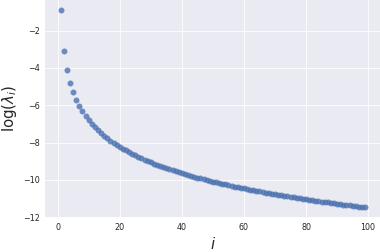
\includegraphics[width=.9\linewidth]{Code/images/12/eigvals}
			\caption{Logarithm of the first 100 eigenvalues of $\K$.}
		\end{subfigure}%
		\begin{subfigure}{.5\textwidth}
			\centering
			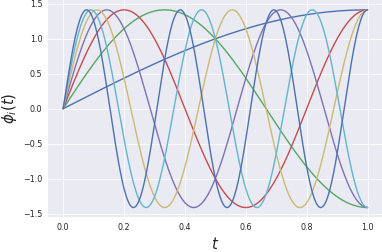
\includegraphics[width=.9\linewidth]{Code/images/12/eigfs}
			\caption{First 7 eigenfunctions of $\K$.}
		\end{subfigure}
		\caption{}
		\label{fig:eigpairwien}
	\end{figure}
	Since $W$ is a Gaussian process, the random variables $xi_i = \langle W,\phi_i\rangle$ are Gaussian in the Karhunen–Loève theorem. Therefore, we can explicitly generate the finite sum approximations $W_n$. An example is shown in Figure \ref{fig:wienerapprox}.
	
	\begin{figure}[h]
		\centering
		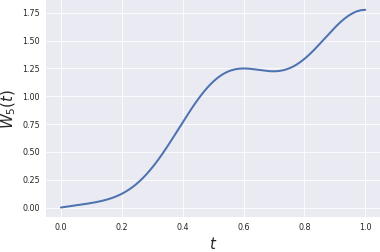
\includegraphics[width=.4\textwidth]{Code/images/12/approx6}\quad
		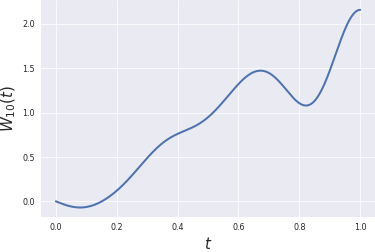
\includegraphics[width=.4\textwidth]{Code/images/12/approx11}
		
		\medskip
		
		
		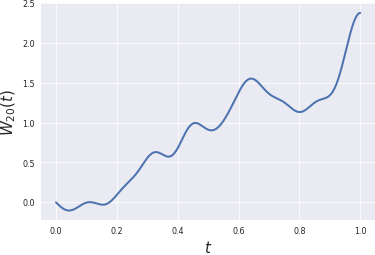
\includegraphics[width=.4\textwidth]{Code/images/12/approx21}
		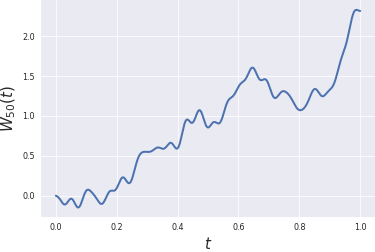
\includegraphics[width=.4\textwidth]{Code/images/12/approx51}
		
		\medskip
		
		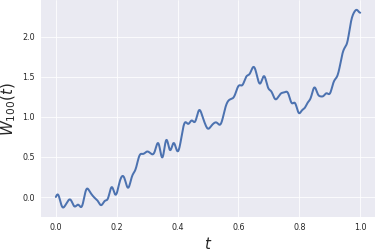
\includegraphics[width=.4\textwidth]{Code/images/12/approx101}\quad
		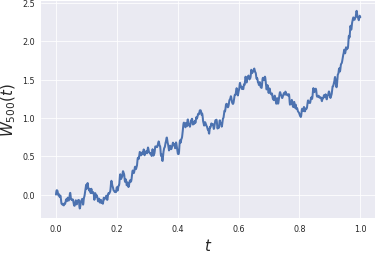
\includegraphics[width=.4\textwidth]{Code/images/12/approx501} \quad
		
		\caption{Finite sum approximations $W_n$ of $W$ for $n=5,10,20,50,100,500$.}
		\label{fig:wienerapprox}
	\end{figure}
\end{ex}
Two of the most important theorems in classical statistics are the strong law of large numbers and the central limit theorem. Fortunately, these two results still hold in the functional setting. We state them here without proof, which can be found in \cite[Theorem 7.7.2 and 7.7.6]{found}.
\begin{theorem}[Strong law of large numbers] 
		Let $\{X_i\}_{i=1}^\infty$ be a sequence of i.i.d stochastic processes with $\E\Vert X_1 \Vert_{\Ll^2}<\infty$ and $\E[X_1]=\mu$. Let $S_n=X_1 +...+X_n$ be the sequence of partial sums. Then,
		$$\frac{S_n}{n} \ \stackrel{a.s.}{\longrightarrow} \ \mu.$$  
\end{theorem}
\begin{theorem}[Central limit theorem]
	Let $\{X_i\}_{i=1}^\infty$ be a sequence of i.i.d stochastic processes with $\E\Vert X_1 \Vert^2_{\Ll^2}<\infty$, $\E[X_1]=\mu$ and covariance operator $\K$. Then,
	$$\frac{1}{\sqrt{n}}\sum_{i=1}^{n}(X_i-\mu) \ \stackrel{dist}{\longrightarrow} \ N_{0,\K},$$
	where $N_{0,\K}$ denotes a Gaussian measure om $\Ll^2[0,1]$, meaning that for any $f\in \Ll^2[0,1]$,
	$$\left\langle f, \frac{1}{\sqrt{n}}\sum_{i=1}^{n}(X_i-\mu)\right\rangle \ \stackrel{dist}{\longrightarrow} \ N_{0,\langle\K f,f\rangle},$$
	see Chapter \ref{chap:gauss}.
\end{theorem}

\section{Statistical analysis of functional data}
We now take on the task of estimating some parameters of a process from observing a finite sample. Our exposition follows that of \cite{inference}. Our setup will be as follows. We observe $N$ i.i.d. samples $X_1,...,X_N$ coming from a second-order mean-squared continuous process. In this section, we will see how to estimate the mean, covariance kernel and eigenpairs of the covariance operator of this process.\\
We start with the mean $\mu = \E[X_1]$. As in the finite dimensional setting, we estimate it using the sample mean 
$$\hat{\mu}(t) = \frac{1}{N}\sum_{i=1}^{N} X_i(t).$$
The next theorem shows that $\hat{\mu}$ is a unbiased $\Ll^2$-consistent estimator.
\begin{theorem}\label{consmu}
	The process $\hat{\mu}$ satisfies $\E[\hat{\mu}]=\mu$ and 
	$$\E\Vert \hat{\mu}-\mu \Vert^2 = O\left(\frac{1}{N}\right).$$
	Moreover, 
	$$\sqrt{n}(\hat{\mu}-\mu) \stackrel{dist}{\longrightarrow} \ N_{0,\K}.$$ 
	\begin{proof}
		For any $t\in [0,1]$, 
		$$\E[\hat{mu}(t)]=\frac{1}{N}\sum_{i=1}^{N}\E[X_i(t)]=\mu(t),$$
		whence $\E[\hat{\mu}]=\mu$. 
		We note that $\hat{\mu}-\mu = N^{-1}\sum_{i=1}^{N}(X_i-\mu)$, so that 
		$$\E\Vert \hat{\mu}-\mu \Vert^2 = \frac{1}{N^2}\sum_{i,j=1}^{N}\E\left[\langle X_i-\mu,X_j-\mu \rangle \right]=\frac{1}{N^2}\sum_{i=1}^{N}\E\left[\langle X_i-\mu,X_i-\mu \rangle \right] = \frac{1}{N} \E\Vert X_1-\mu \Vert^2 = O\left(\frac{1}{N}\right),$$
		where we used that $X_i$ and $X_j$ are independent for $i\ne j$, so that 
		$$\E\left[\langle X_i-\mu,X_j-\mu \rangle \right] = 0.$$
		The last statement follows immediately from the central limit theorem.
	\end{proof}
\end{theorem}
The estimation of the covariance kernel is also performed similarly to the finite dimensional setting. We estimate it with 
$$\hat{K}(s,t) = \frac{1}{N}\sum_{i=1}^{N}(X_i(s)-\hat{\mu}(s))(X_i(t)-\hat{\mu}(t)).$$
As in the finite dimensional case, this estimator is biased with 
$$\E[\hat{K}(s,t)] = \frac{N-1}{N}K(s,t),$$
which is negligible when $N$ is large. We estimate the covariance operator by the induced operator of $\hat{K}$, i.e., with
$$\hat{\K} f(t) = \int_{0}^{1} \hat{K}(s,t)f(s)ds = \frac{1}{N}\sum_{i=1}^{N}(X_i(t)-\hat{\mu}(t))\langle X_i-\hat{\mu}, f \rangle.$$
This last expression shows that the range of $\hat{\K}$ is contained in the span of $\{X_1,...,X_N\}$ and is thus finite dimensional. This is the source of many problems in functional data analysis, since the true covariance operator is often infinite dimensional.\\
To analyze this estimator, we need to choose an operator space in which we can work. As was shown in Theorem \ref{propcovop}, the true covariance operator $\K$ lives in the spaces of bounded, Hilbert-Schmidt and trace class operators. We note that $\hat{\K}$ also belongs to these spaces since it has finite dimensional range. Of those, the space of Hilbert-Schmidt operators $\mathcal{S}(\Ll^2[0,1])$ is the most convenient since it is itself a separable Hilbert space which makes the computations easier. To make them even easier, we assume that $\mu \equiv \hat{\mu} \equiv 0$. This assumption is not too optimistic in practice since $\hat{\mu}$ converges quite rapidly to $\mu$. The next theorem shows that $\hat{\K}$ has good properties.
\begin{theorem}
	If $\E\Vert X_1\Vert^4 < \infty$, the estimator $\hat{\K}$ satisfies:
	\begin{enumerate}
		\item $\hat{\K} \ \stackrel{a.s.}{\longrightarrow} \ \K$,
		\item $\E\Vert \hat{\K}-\K \Vert^2_{HS} \leq \frac{1}{N}\E\Vert X_1\Vert^4$,
	\end{enumerate}
	\begin{proof}
		\begin{enumerate}
			\item As noted above, $\hat{K}$ can be written as $N^{-1}\sum_{i=1}^{N}X_i\langle X_i,\cdot \rangle$. Consider the operators 
			$$\K_i = X_i\langle X_i,\cdot \rangle - \K, \ i=1,...,N.$$
			Then, $\hat{\K} -\K = N^{-1}\sum_{i=1}^{N}\K_i$ and $\E[\K_i]=0$ for $i=1,...,N$. Therefore, by the strong law of large numbers,
			$$\hat{\K}-\K \stackrel{a.s}{\longrightarrow} 0 \ \iff \ \hat{\K} \stackrel{a.s}{\longrightarrow} \K.$$
			\item Let $\{\phi_k\}$ is a complete orthonormal system of $\Ll^2[0,1]$,
			$$\Vert X_i\langle X_i,\cdot \rangle\Vert_{HS}^2 = \sum_{k=1}^{\infty}\Vert X_i\langle X_i,\phi_k\rangle \Vert^2 = \Vert X_i \Vert^2 \sum_{k=1}^{\infty}\langle X_i,\phi_k\rangle^2 = \Vert X_i \Vert^4.$$
			Then, by similar computations as those carried out in the proof of Theorem \ref{consmu}, one can show that (see \cite[Theorem 2.5]{inference})
			$$\E\Vert \hat{\K}-\K \Vert^2_{HS} = \E\left\langle \frac{1}{N}\sum_{i=1}^{N} \K_i,\frac{1}{N}\sum_{i=1}^{N} \K_i \right\rangle_{HS} \leq \E\Vert X_1\Vert^4.$$
		\end{enumerate}
	\end{proof}
\end{theorem}
One of the most popular tool in functional data analysis is the functional principal component analysis (FPCA) method. This method uses the Karhunen-Loève theorem to reduce the dimension of the data to infinite to finite. Similarly to the PCA method in multivariate analysis, we approximate the process $X$ using only the $r$ principal components (we still assume $\E[X]\equiv 0$):
$$X \simeq X^r = \sum_{i=1}^{r}\xi_i \phi_i.$$
The process $X^r$ has covariance operator $\K^r = \sum_{i=1}^{r}\lambda_i \phi_i \otimes \phi_i$ and therefore ``explain'' a ratio of 
$$\frac{\mathrm{Tr}(\K^r)}{\mathrm{Tr}(\K)} = \frac{\sum_{i=1}^{r}\lambda_i}{\sum_{i=1}^{\infty}\lambda_i}$$
of the variance of $X$.\\
In practice, one does not have access to the eigenpairs $\{\lambda_i,\phi_i\}_{i=1}^r$ of $\K$ and we thus need a way to approximate them. The obvious way to do so is by using the eigenpairs $\{\hat{\lambda}_i,\hat{\phi}_i\}_{i=1}^r$ of $\K$. We assume that $\lambda_1>...>\lambda_r>0$ to make the problem identifiable. Moreover, we assume that we can the estimates $\hat{\phi_i}$ have good signs, i.e., that $\langle \phi_i,\hat{\phi_i}\rangle\geq 0$ for all $i$. In practice, one is only interested in the eigenspaces, so this last assumption is not to restrictive.\\
Then, the next theorem, proved in \cite[Section 2.7]{inference}, shows that $\{\hat{\lambda}_i,\hat{\phi}_i\}_{i=1}^r$ are consistent estimators of $\{\lambda_i,\phi_i\}_{i=1}^r$.
\begin{theorem}
	Suppose $\E\Vert X_1 \Vert^4 < \infty$, $\lambda_1>...>\lambda_r>0$, and $\langle \phi_i,\hat{\phi_i}\rangle\geq 0$ for all $i$. Then, for all $i=1,...,r$,
	$$\limsup_{N\to \infty} N \E\Vert \hat{\phi}_i - \phi_i\Vert^2 < \infty \ \text{ and } \ \limsup_{N\to \infty} N \E\vert \hat{\lambda}_i - \lambda_i\vert^2 < \infty.$$
\end{theorem}
Consequently, given a new observation $\tilde{X}$ one can estimate the component scores $\langle \tilde{X}, \phi_i\rangle \sim \xi_i$ with $\langle \tilde{X}, \hat{\phi}_i\rangle$ and get 
$$\sup_{i=1...r}\E\left( \langle \tilde{X}, \hat{\phi}_i\rangle - \langle \tilde{X}, \phi_i\rangle\right)^2 = \sup_{i=1...r}\E\langle \tilde{X}, \hat{\phi}_i-\phi_i\rangle^2 \leq \sup_{i=1...r}\E\Vert \tilde{X}\Vert^2 \Vert \hat{\phi}_i-\phi_i\Vert^2 \stackrel{N\to \infty}{\longrightarrow} 0.$$

\section{Discrete observations and smoothing}
In practice, curves are never observed on their full domain, they are observed on a finite discrete subset $\{t_1,...,t_k\}$. Moreover, each observation can be subject to measurement errors. Therefore, in practice the observations are of the form:
$$X_{ij}=X_i(t_j) + \epsilon_{ij}, \ i=1,...,N,\ j=1,...,K,$$
where the $\epsilon_{ij}$ are i.i.d, of mean 0 and variance $\sigma^2$ and independent of the $X_i$'s.\\
To be able to work with functional data, the full curves $X_i$ need to be approximated. This can be done by smoothing either the observations themselves or the covariance kernel.\\
To smooth the observations, a popular approaches is the penalized smoothing method. One first needs to choose a function space $\mathbb{W}$ in which we want our approximations to live, and a penalty function $P:\mathbb{W}\to \R_+$ that penalizes unwanted behaviors. Then, we approximate $X_i$ with 
$$\tilde{X}_i = \arg\min_{f \in \mathbb{W}}\left[ \sum_{j=1}^{K}(X_i(t_j)-f(t_j))^2 + \lambda P(f) \right],$$ 
where $\lambda >0$ is a tuning parameter. A popular choice for $\mathbb{W}$ and $P$ are 
$$\mathbb{W}=C^2[0,1] \ \text{ and } \ P(f) = \int_{0}^{1}\left\vert \frac{d^2 f}{dt^2}(t)\right\vert^2 dt.$$
With this choice, we ask for our approximation to be twice differentiable and not to be too rough. Moreover, one can show that an explicit solution can be found in terms of cubic splines. For more details, see \cite[Chapter 5]{fdaram}. Using the smooth estimates $\tilde{X}_1,...,\tilde{X}_N$, the mean and covariance kernel can be estimated, as explained in the previous section.\\
When the observation grid $\{t_1,...,t_K\}$ is sparse, the penalized smoothing approach will typically yield biased estimates. In that case, a popular approach is the PACE method described in \cite{pace}. In this method, one starts by estimating the covariance kernel. This is done by smoothing the covariance matrix of the observations $X_{ij}$, $i=1,...,N$, $j=1,...,K$, where the diagonal is removed to take care of the noise $\epsilon_{ij}$. Then, eigenpairs of the covariance operator are estimated by $\{\hat{\lambda_k},\hat{\phi_k}\}$, the eigenpairs of the estimated smoothed covariance kernel. Finally, the components scores $\xi_{ik} = \langle X_i, \phi_k\rangle$ are estimated using the explicit formulat for the conditional expectation in the Gaussian case:
$$\hat{\xi}_{ik} = \widehat{\E}[\xi_{ik}\mid X_i(t_1),...,X_i(t_K)].$$
The full curves $X_i$ are then estimated using the FPCA method:
$$X_i= \hat{\mu} + \sum_{k=1}^{r} \hat{\xi}_{ik} \hat{\phi}_{k}.$$
This method is shown to have better asymptotic properties when the observations are sparse.
\begin{ex}
	We illustrate the methods above with the growth data set of \cite{growth}, shown in Figure \ref{fig:growth}. We focus only on boys, for which there are 39 samples observed at 95 regularly sampled ages. We start by smoothing the observations using cubic splines. We then compute the derivatives of these smooth estimates. These derivatives are shown in the top left of Figure \ref{fig:exfpca}. We then compute the principal components using the eigenpairs of the estimated covariance kernel. The first three principal components explain 85\% of the total variance. In the top right and bottom of Figure \ref{fig:exfpca}, we show the mean derivative in blue, along with the curves
	$$\hat{\mu} \pm 2\sqrt{\lambda_i}\phi_i, \ i=1,2,3$$
	in red. We see that the first principal component explains two main modes of variation, one between 8 and 13, and the other between 16 and 18. Individuals having a high positive score in this component typically experience their puberty earlier and have a big spike in their growth around 12 years old. On the other hand, individuals having a high negative score in this component will experience puberty later, around 15 years old. The second component deals mainly with the variation close to birth. The third component is more difficult to interpret and is similar to the first component.
	\begin{figure}[H]
		\centering
		\begin{subfigure}{.4\textwidth}
			\centering
			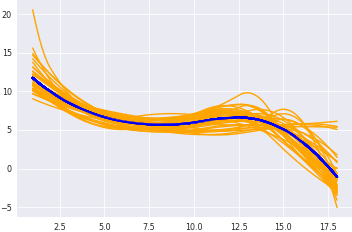
\includegraphics[width=.8\linewidth]{Code/images/14/boys}
			\caption{Derivatives with mean in blue.}
		\end{subfigure}%
		\begin{subfigure}{.4\textwidth}
			\centering
			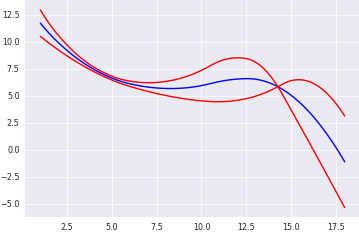
\includegraphics[width=.8\linewidth]{Code/images/14/pca1}
			\caption{\centering First component.}
		\end{subfigure}
		
		
		\medskip
		
		
		\begin{subfigure}{.4\textwidth}
			\centering
			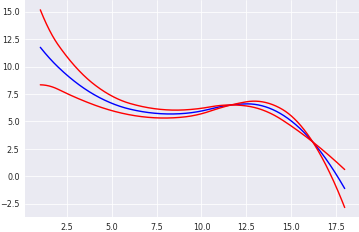
\includegraphics[width=.8\linewidth]{Code/images/14/pca2}
			\caption{\centering Second component.}
		\end{subfigure}%
			\begin{subfigure}{.4\textwidth}
				\centering
				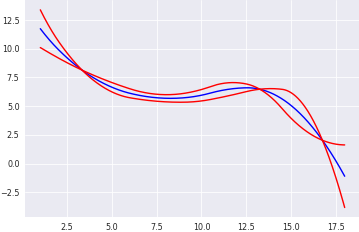
\includegraphics[width=.8\linewidth]{Code/images/14/pca3}
				\caption{\centering Third component.}
			\end{subfigure}
		\caption{Example of FPCA on the growth data set.}
		\label{fig:exfpca}
	\end{figure}
	This example shows how FPCA can be used to analyze the variation of a population of curves.\\
	We note that our analysis is rather shallow since it does not take care of the time-registration problem. A thorough analysis of this dataset is performed in \cite[Chapter 6]{apfda}
\end{ex}
\chapter{Censored functional data}\label{chap:frags}
\section{Functional fragments framework}\label{introfrag}
\textit{Censored functional data} or \textit{functional fragments} are functional data that are not observed in the full domain on which they are defined. If the data live in $\Ll^2(\mathcal{I})$ for some interval $\mathcal{I} \subset \R$, an example of functional fragment is a function $f \in \Ll^2(\mathcal{J})$ for some interval $\mathcal{J}\subset \mathcal{I}$.

By the \textit{functional fragments framework}, we mean the statistical framework in which some or all of the observed data are in the form of fragments of some underlying, unobservable, functional data. In this case, the data at hand are pairs $\{(X_i,\mathcal{O}_i)\}_{i=1}^n$, where the $X_i$'s are random functions in $\Ll^2(\mathcal{O}_i)$ for some subintervals $\mathcal{O}_i$. We will often assume that the subintervals $\{\mathcal{O}_i\}_{i=1}^n$ are themselves random, in order to make the asymptotic theory more tractable. This framework often arises in practice when an observation is unavailable before or after a certain time.\\
The main issue in the functional fragments framework is to know to what extent one can recover precise information on the underlying population from the observed fragments. For example, how precisely can we estimate the mean and covariance when no curve is fully observed.\\
Following \cite{DP2}, we distinguish between two ways in which the intervals $\{\mathcal{O}_i\}_{i=1}^n$ are distributed, see Figure \ref{fig:exfrags}:\\

\noindent
\textbf{1.} A ``blanket '' regime, where the curves are typically observed on most or all of the domain. Then the number of observations at a given point of the domain is close to the total number of observations.\\
\textbf{2.} A ``banded'' regime, where the lengths of the $\mathcal{O}_i$ are bounded by some value $\delta>0$. Then, we have no explicit information on the covariance of points that are at distance larger than $\delta$.
\begin{figure}[ht]
	\centering
	\begin{subfigure}{.3\textwidth}
		\centering
		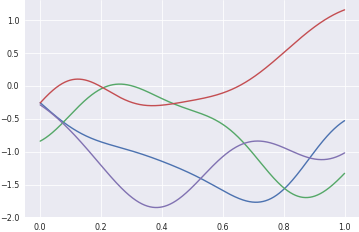
\includegraphics[width=.8\linewidth]{Code/images/21/full}
		\caption{Full curves}
	\end{subfigure}%
	\begin{subfigure}{.3\textwidth}
		\centering
		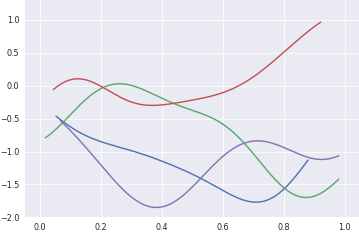
\includegraphics[width=.8\linewidth]{Code/images/21/blanket}
		\caption{\centering Fragments in the blanket regime}
	\end{subfigure}
	\begin{subfigure}{.3\textwidth}
		\centering
		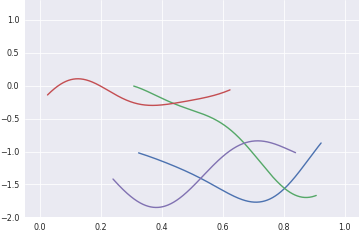
\includegraphics[width=.8\linewidth]{Code/images/21/frags}
		\caption{\centering Fragments in the banded regime}
	\end{subfigure}
	\caption{Example of functional fragments}
	\label{fig:exfrags}
\end{figure}

In the rest of this chapter, we will present various methods used in the literature dealing with those issues. 	

\section{Naive estimations}\label{naiveest}
We present here the methods presented in \cite{Kraus1}. The data are i.i.d curves $X_i$ in $\Ll^2[0,1]$ observed only on a random interval $\mathcal{O}_i \subset [0,1]$, $i=1,...,n$. To estimate the population mean $\mu = \E[X_1]$ and covariance operator $\mathcal{K} = \E[(X_1-\mu) \otimes (X_1-\mu)]$, the unobserved parts of the curves are ignored and the sample estimators are created naively as follows. The sample mean $\hat{\mu}$ is found by taking the mean of the pointwise observed values: 
\begin{equation}\label{estmufrag}
	\hat{\mu}(t) = \frac{\mathbf{1}[\exists \mathcal{O}_i \ni t ]}{\sum_{i=1}^n \mathbf{1}[t \in \mathcal{O}_i]} \sum_{i=1}^n \mathbf{1}[t \in \mathcal{O}_i] \cdot X_i(t).
\end{equation}

The covariance operator is estimated in the same fashion via its associated covariance kernel $K(\cdot,\cdot)$. The sample kernel is given by:
\begin{equation}\label{estcovfrag}
	\hat{K}(s,t) = \frac{\mathbf{1}[\exists \mathcal{O}_i \ni s,t ]}{\sum_{i=1}^n \mathbf{1}[s,t \in \mathcal{O}_i]} \sum_{i=1}^n \mathbf{1}[s,t \in \mathcal{O}_i] \cdot \left\{X_i(s)-\hat{\mu}_{st}(s)\right\}\left\{X_i(t)-\hat{\mu}_{st}(t)\right\},
\end{equation}
where  $\hat{\mu}_{st}$ is an estimation of the mean using only the curves observed at $s$ and $t$:
\[\hat{\mu}_{st}(s) = \frac{\mathbf{1}[\exists \mathcal{O}_i \ni s,t ]}{\sum_{i=1}^n \mathbf{1}[s,t \in \mathcal{O}_i]} \sum_{i=1}^n \mathbf{1}[s,t \in \mathcal{O}_i] \cdot X_i(s). \]
The sample covariance operator $\hat{\mathcal{K}}$ is then defined by 
\[\hat{\mathcal{K}}f(t) = \int_{0}^{1} \! \hat{K}(s,t)f(s) \, \mathrm{d}s.\]
We note that this operator need not be positive-definite. This can be dealt with by clipping the negative eigenvalues to zero.\\
The following proposition, proved in \cite[Prop. \!1]{Kraus1}, shows that under some assumptions on the random intervals $\{\mathcal{O}_i\}_{i=1}^n$, the above estimates enjoy the same asymptotic convergence rate as their counterparts when the curves are fully observed.
\begin{prop}
	\begin{itemize}
		\item[]
		\item[1.] Suppose that $\mathbb{E}\Vert X_1\Vert^2<\infty$ and the $\mathcal{O}_i$'s are i.i.d with $\inf_{t \in [0,1]} \Pp\left[t \in \mathcal{O}_1\right]>0$. Then 
		\[\mathbb{E}\Vert \hat{\mu}-\mu\Vert^2 = O(n^{-1}) \text{ as } n \to \infty. \]
		\item[2.] Suppose further that $\mathbb{E}\Vert X_1\Vert^4<\infty$ and that $\inf_{s,t \in [0,1]} \Pp\left[s,t \in \mathcal{O}_1\right]>0$. Then 
		\[\mathbb{E}\Vert \hat{\mathcal{K}}-\mathcal{K}\Vert^2_{HS} = O(n^{-1}) \text{ as } n \to \infty. \]
	\end{itemize}
	\qed
\end{prop}
For the covariance operator, even though the theoretical convergence rate is good, in practice the estimate is not adequate in the ``banded'' regime (see Section \ref{introfrag}). The problem is that in this regime, the estimated kernel is necessarily zero in the region $\{(s,t)\in [0,1]^2 \, \mid \, \vert s-t\vert > \delta \}$. This problem that is not present in the ``blanket'' regime, as soon as one full curve is observed, see Figure .
\begin{figure}[H]
	\centering
	\begin{subfigure}{.3\textwidth}
		\centering
		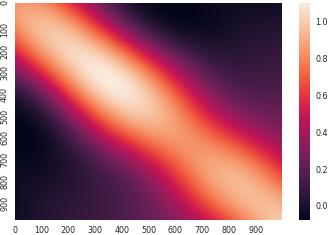
\includegraphics[width=.8\linewidth]{Code/images/22/truecov}
		\caption{Full curves}
	\end{subfigure}%
	\begin{subfigure}{.3\textwidth}
		\centering
		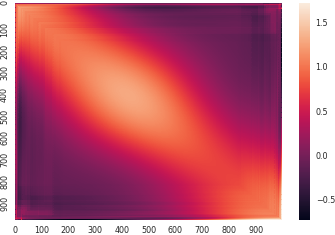
\includegraphics[width=.8\linewidth]{Code/images/22/blanketheat}
		\caption{\centering Fragments in the blanket regime}
	\end{subfigure}
	\begin{subfigure}{.3\textwidth}
		\centering
		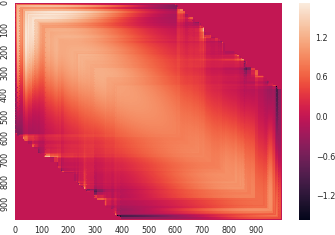
\includegraphics[width=.8\linewidth]{Code/images/22/fragsheat}
		\caption{\centering Fragments in the banded regime}
	\end{subfigure}
	\caption{Sample estimates of the covariance kernel in the different regimes}
	\label{fig:excov}
\end{figure}

\section{Curve extension}\label{sec:curveext}
In \cite{DH1}, the authors take the approach of manually extend the fragments by gluing some of their parts. This procedure is carried on in the context of classification, but it can readily be expended to the plain estimation of the population mean and covariance.\\
The extension of a fragment to the right is done by iteratively gluing a small section of another randomly chosen nearby fragment to the right endpoint of the original fragment. Likewise for the extension to the left. A few steps of this procedure are shown in Figure \ref{fig:gluingsteps}.
\begin{figure}[htp]
	\centering
	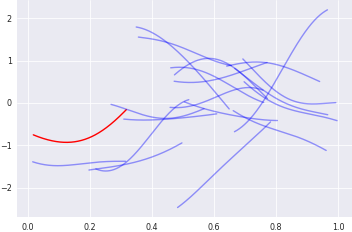
\includegraphics[width=.4\textwidth]{Code/images/23/step1}\quad
	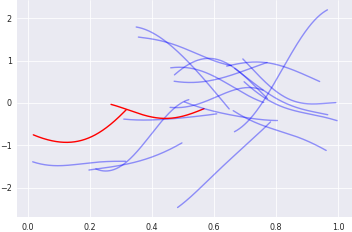
\includegraphics[width=.4\textwidth]{Code/images/23/step2}\quad
	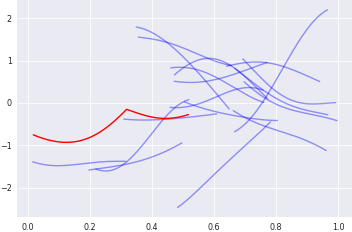
\includegraphics[width=.4\textwidth]{Code/images/23/step3}
	
	\medskip
	
	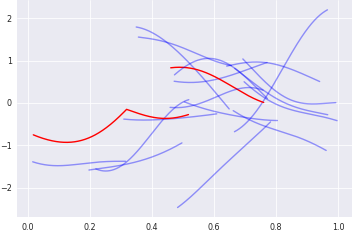
\includegraphics[width=.4\textwidth]{Code/images/23/step4}\quad
	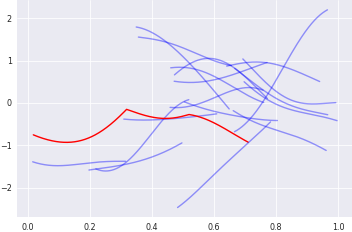
\includegraphics[width=.4\textwidth]{Code/images/23/step5}
	
	\caption{Illustration of a few steps of the gluing procedure}
	\label{fig:gluingsteps}
\end{figure}

In this way, for each fragment $(X_i, \mathcal{O}_i)$, one gets a curve $\tilde{X}_i$ defined on the entire domain. From these full curves, the sample mean and covariance can be estimated. This estimation method works both in the ``blanket'' and the ``banded'' regime, since in both cases full curves are constructed. Examples of those estimates are shown in Figure \ref{fig:gluingex}.\\
\begin{figure}[ht]
	\centering
	\begin{subfigure}{.4\textwidth}
		\centering
		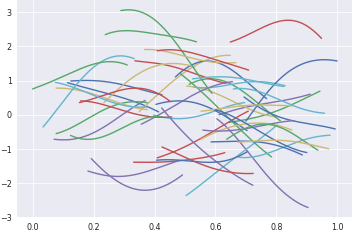
\includegraphics[width=.8\linewidth]{Code/images/23/frags}
		\caption{Fragments}
	\end{subfigure}%
	\begin{subfigure}{.4\textwidth}
		\centering
		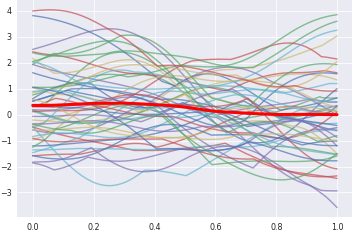
\includegraphics[width=.8\linewidth]{Code/images/23/extended}
		\caption{\centering Reconstructed curves with their mean in red}
	\end{subfigure}
	
	
	\medskip
	
	
	\begin{subfigure}{.4\textwidth}
		\centering
		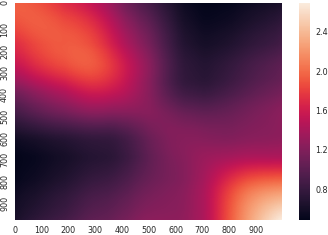
\includegraphics[width=.8\linewidth]{Code/images/23/cov}
		\caption{\centering Estimated covariance kernel form the reconstructed curves }
	\end{subfigure}
	\caption{Example of mean and covariance estimation using the gluing procedure}
	\label{fig:gluingex}
\end{figure}
To the best of our knowledge, no theoretical convergence rates for these estimates have been found. We also note that another function extension method for functional fragments is presented in \cite{DH2} by the same authors. This method assumes that discretized versions of the curves are Markov processes and then extend the fragments using this assumption.



\section{Covariance recovery}
In this section, we present the covariance recovery method of \cite{DP2}. In this paper, the authors show that under some smoothness assumptions, one can use a matrix completion method to recover the covariance matrix of a process from the observations of fragments in the ``banded'' regime. 
\subsection{Setup}\label{recovsetup}
We consider a continuous stochastic process $X \in \Ll^2[0,1]$ with mean function $\E[X]=\mu$ and covariance kernel $r(s,t) = \text{cov}\! \left\{ X(s) , X(t) \right\}$. Suppose we observe i.i.d. fragments $(X_i,\mathcal{O}_i)$ of length $\delta \in (0,1)$. Then, one can compute the estimates $\tilde{\mu}_n$ and $\tilde{r}_n$ given by Equations \ref{estmufrag} and \ref{estcovfrag}. Suppose further that we observe these fragments only on a grid of size $K$
\[ (t_1,...,t_K) \in \mathcal{T}_K = \{(x_1,...,x_K)\in \R^K \, \mid \, x_i \in I_{i,K} \}, \]
where $\{I_{i,K}\}_{i=1}^K$ is the regular partition of $[0,1]$ in intervals of length $1/K$. From these discrete observations, one can compute the mean vector $\tilde{\mu}_n^K = (\tilde{\mu}_n(t_i))_{i=1}^K$ and the covariance matrix $\tilde{R}_n^K = \{\tilde{r}_n(t_i,t_j)\}_{i,j=1}^K$. As noted above, this matrix will have a banded structure. Indeed, each fragment $X_i$ is observed only on $\mathcal{O}_i \cap \{t_i\}_{i=1}^K$, which has between $\lfloor{K\delta}\rfloor -1$ and $\lceil{K\delta}\rceil +1$ points. Thus, the matrix $\tilde{R}_n^K$ is guaranteed to have non-zero values only on the band $\{(i,j) \, \mid \, \vert i-j\vert < \lfloor{K\delta}\rfloor -1\}$. Denote by $R^K$ the true covariance matrix $\{r(t_i,t_j)\}_{i,j=1}^K$ and by $P_\delta^K \in \R^{K \times K}$ the band indicator matrix 
$$P_{\delta}^K(i,j) = \mathbf{1}\left[\, \vert i-j\vert < \lfloor{K\delta}\rfloor -1\right].$$
Then $\tilde{R}_n^K$ can realistically be seen only as an estimator of $P_{\delta}^K \circ R^K$, where ``$\circ$'' denotes the Hadamard product. \\
The question now is, under what non-parametric conditions on the process $X$ one can hope to efficiently recover the full covariance matrix $R^K$ from its banded version $P_{\delta}^K \circ R^K$? The estimation of the covariance in this setup can thus be seen as a matrix completion problem. 

\subsection{Identifiability and estimation}
The main result of \cite{DP2} is that under simple non-parametric assumptions given below, one can exactly recover the covariance matrix from its banded version. Moreover, they show that these condtions are, in some sense, necessary. These assumptions are the following:
\begin{itemize}
	\item[1.] The covariance kernel $r(s,t)$ has finite rank $q$, i.e., it admits a Mercer decomposition 
	$$r(s,t) = \sum_{j=1}^{q} \lambda_j \phi_j(s)\phi_j(t).$$
	\item[2.] The eigenfunctions $\{\phi_1,...,\phi_q\}$ are all real analytic.
\end{itemize}
The following results, shown in \cite[Prop.\! 1]{DP1}, indicate that the second condition is not as strict as it seems.

\begin{prop}
	The set of trace class covariance operators of rank at most $q$ with analytic eigenfunctions is dense in the space of rank $q$ trace class covariance operators with the nuclear norm. In particular, for any process $X  \in \Ll^2[0,1]$ with finite rank $q$ trace class operator and any $\epsilon>0$, there exists a process $Y$, satisfying the conditions above, such that 
	$$\E\Vert X-Y\Vert^2_{\Ll^2} < \epsilon.$$ \qed
\end{prop}

The main property of finite rank analytic kernel we will use is the one known as analytic continuation. We will need it in the following form, which is a special case of \cite[Corollary 1.2.6]{analprimer}:
\begin{prop}
	Let $r,l:[0,1]^2 \to \R$  be two real analytic finite rank kernels. Suppose that there exists an open set $U \subseteq [0,1]^2$ such that $r(s,t)=l(s,t)$ for all $(s,t)\in U$. Then $r(s,t)=l(s,t)$ for all $(s,t) \in [0,1]^2$, i.e., $r$ and $l$ are equal. \qed
\end{prop}
In our setup, this implies that knowing the covariance kernel on the band $\{(s,t) \in [0,1]^2 \ \mid \ \vert s-t \vert < \delta\}$ allows us to recover the kernel on the whole domain $[0,1]^2$. This shows that the model is identifiable in the sense that one can recover the true covariance from the observations of fragments. \\
In the discretized setup, this translates into the following identifiability result:
\begin{theorem}[\cite{DP2}]
	Suppose that the covariance kernel $r(s,t)$ is analytic of finite rank $q$. If $\delta$ and $K$ are such that 
	$$K>\frac{q+2}{\delta}$$
	then, for almost all $(t_1,...,t_K) \in \mathcal{T}_K$, then the covariance matrix $R^K$ is the unique solution of 
	\begin{equation}\label{matcomp}
		\min_{M \in \R{K \times K}} \text{rank}(M) \ \text{ subject to } \ \Vert P_\delta^K \circ (R^K - M) \Vert_{Frob}=0.
	\end{equation}

	Equivalently, introducing a Lagrange multiplier, for all $\tau>0$ sufficiently small,
	\[R^K = \underset{M \in R^{K\times K}}{\text{argmin}} \left\{\Vert P_\delta^K \circ (R^K - M) \Vert_{Frob}^2 + \tau \, \text{rank}(M) \right\} \]
	almost everywhere on $\mathcal{T}_K$.
	\begin{proof}
		By \cite[Theorem 4]{DP1}, all $q\times q$ minors of $R^K$ are non-zero. Moreover, the condition $K>(q+2)/\delta$ implies that $R^K$ and $P_\delta^K \circ R^K$  share at least one common $q\times q$  submatrix. Combining these two results yields that $R^K$ has rank $q$ and that $P_\delta^K \circ R^K$ has rank at least $q$. Therefore $R^K$ is a solution of the matrix completion problem \ref{matcomp}. It remains to show that it is the unique solution thereof. Let $R^*$ be another solution. Then, by design, $R^*$ has rank $q$ and is equal to $R^K$ on the band $B_\delta=\{(i,j) \, \mid \, \vert i-j\vert < \lfloor{K\delta}\rfloor -1\}$. Since $K>(q+2)/\delta$, we can find a $(q+1)\times (q+1)$ submatrix $A$ of $R^*$ with exactly one entry $x^*$ outside the band $B_\delta$, see Figure \ref{fig:matcomp}.
		\begin{figure}[ht]
		\centering
		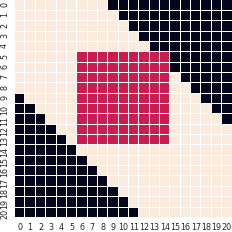
\includegraphics[width=0.5\linewidth]{Code/images/24/matcomp}
		\caption{Illustration of the matrix completion method with $K=21$, $q=8$, $\delta=0.5$. The band $B_\delta$ is colored in white and a possible $(q+1)\times (q+1)$ submatrix $A$ is colored in red.}
		\label{fig:matcomp}
		\end{figure}
		The determinant of $A$ can then be written as $ax^* + b$ where $a$ is the determinant of a $q\times q$ submatrix contained in $B_\delta$, and is thus non-zero, and $b$ depends only on the values of $R^*$ in $B_\delta$. Since $R^*$ has rank $q$, $$\det(A)=ax^*+b=0.$$ 
		Therefore, $x^*$ is uniquely determined by the values of $R^*$ in $B_\delta$, and they are themselves fixed to be equal to the values of $R^K$ in that band. Therefore, all solutions of \ref{matcomp} are equal on the entry $x^*$.\\
		One can iterate this procedure to reconstruct entirely the matrix $R^K$. The solution of \ref{matcomp} is thus unique and given by $R^K$. 
	\end{proof}
	By pluging-in the banded estimator $\tilde{R}_n$ defined in Section \ref{recovsetup}, the theorem naturally leads to the following estimator of the full matrix $R^K$:
	\begin{definition}
		Define the estimator $\hat{R}_n^K$ of $R^K$ as a minimum of 
		\begin{equation}
			\underset{0 \preceq M \in R^{K\times K}}{\text{argmin}} \left\{\Vert \tilde{R}_n^K - P_\delta^K \circ  M \Vert_{Frob}^2 + \tau_n \, \text{rank}(M) \right\},
		\end{equation}
		where $\tau_n$ is a parameter that should converge to 0 as $n$ goes to infinity. From this estimator of the covariance matrix, one can estimate the covariance kernel by the step function
		\begin{equation}
			\hat{r}_n(s,t) = \hat{R}_n^K(i,j) \ \text{ if } \ (s,t)\in I_{i,K}\times I_{j,K}.
		\end{equation}
		\qed
	\end{definition}
\end{theorem}
We have the following consistency result.
\begin{theorem}
	Assume $\E\Vert X_i \Vert^4_{\Ll^2} < \infty$, the intervals $\{\mathcal{O}_1,...,\mathcal{O}_n\}$ are i.i.d. independent of the $X_i$'s and that $\inf_{s,t \in [0,1]} \Pp\left[s,t \in \mathcal{O}_1\right]>0$. Let $K^*= \lfloor (q+2)/\delta\rfloor + 1$ be the critical resolution. Then, if $\tau_n \to 0$, for almost any grid in $\mathcal{T}_K$, 
	\begin{equation}
		\int\int_{[0,1]^2}  \left(\hat{r}_n^K(x,y)-r(x,y)\right)^2 dxdy \leq O_{\Pp}(1/n) + 4K^{-2} \sup_{x,y \in [0,1]} \Vert \nabla r(x,y)\Vert_2^2,
	\end{equation}
	uniformly in $K$, for any refinement $K=m\times K^*$.\qed
\end{theorem}

\subsection{Numerical implementation}
The implementation of the estimator $R^K_n$ is explained in detail in \cite[Section 5]{DP2}. Roughly, it consists of two steps:
\begin{itemize}
	\item[1.] Find an approximate minimum $M_i$ of 
	$$\min_{0\preceq M \in \R^{K\times K}} \Vert \tilde{R}_n^K - P_{\delta}^K \circ M||^2_{Frob} \text{ subject to rank}(M)\leq i $$ 
	for $i \in \{1,...,\lceil K\delta\rceil-3 \}$. This can be done by writing $M_i = \gamma \gamma^T$ with $\gamma \in \R^{K\times i}$ and optimizing on $\gamma$ using general purpose optimization algorithm, e.g., BFGS. Note that the objective function is not convex in $\gamma$. However, numerical experiments indicate that local minima are good enough.
	\item[2.] Compute the objective value $f(i)$ of $M_i$ for all $i \in \{1,...,\lceil K\delta\rceil-3 \}$ and take $\hat{R}_n^K = M_j$ for the rank $j$ after which the function $f$ does not decrease much more.
\end{itemize}

\subsection{Example}
We present here a numerical example of the covariance recovery method. Let $r'(s,t)=\min(s,t)$ be the covariance kernel of the brownian motion and $r(s,t)$ be its projection on its first 10 eigenfunctions. Then $r(s,t)$ is a rank $10$ analytic kernel. We take $\mu \equiv 0$, $n=100$, $K=50$, $\delta=0.6$ in the following. Example of fragments along with the estimated mean $\tilde{\mu}_n^K$ are shown in Figure \ref{fig:fragex}.
\begin{figure}
\centering
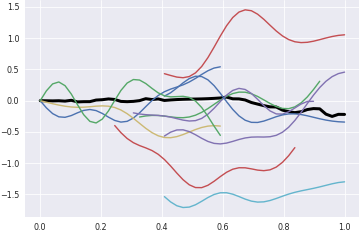
\includegraphics[width=0.7\linewidth]{Code/images/24/fragex}
\caption{Plot of 10 fragments (out of the total 100), and the estimated mean in black. }
\label{fig:fragex}
\end{figure}
The true covariance matrix $R^K$ along with the banded estimator $\tilde{R}_n^K$ are shown in Figure \ref{fig:truetrunccov}.
\begin{figure}[H]
	\centering
	\begin{subfigure}{.5\textwidth}
		\centering
		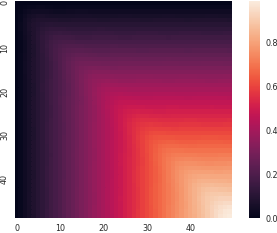
\includegraphics[width=.8\linewidth]{Code/images/24/truecov}
		\caption{True covariance matrix}
	\end{subfigure}%
	\begin{subfigure}{.5\textwidth}
		\centering
		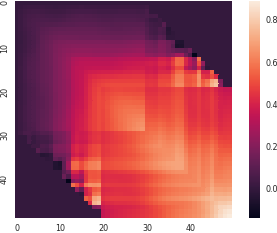
\includegraphics[width=.8\linewidth]{Code/images/24/trunccov}
		\caption{Banded estimator}
	\end{subfigure}
	\caption{}
	\label{fig:truetrunccov}
\end{figure}
The relative error $\Vert R^K - \tilde{R}_n^K\Vert / \Vert R^K \Vert$ is 27.2\% here. We now perform the first step of the implementation, as described in the previous section. A plot of the objective values for $i \in \{1,...,10\}$ is shown in Figure \ref{fig:obvals}.
\begin{figure}
\centering
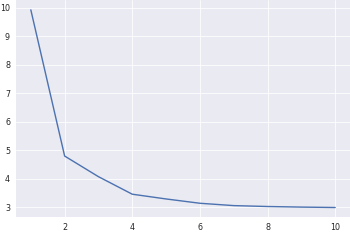
\includegraphics[width=0.7\linewidth]{Code/images/24/obvals}
\caption{Objective value in function of the rank.}
\label{fig:obvals}
\end{figure}
From this plot, we decide to choose the rank of the estimator to be $i=5$. The resulting estimator $\hat{R}_n^K = M_5$  is shown in Figure \ref{fig:estcov}.
\begin{figure}
\centering
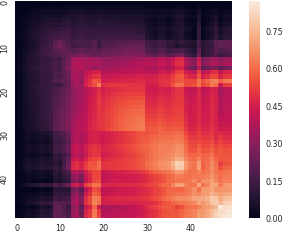
\includegraphics[width=0.7\linewidth]{Code/images/24/estcov}
\caption{Estimated covariance matrix $\hat{R}_n^K$.}
\label{fig:estcov}
\end{figure}
The relative error with this estimate is $\Vert R^K - \hat{R}_n^K\Vert / \Vert R^K \Vert = 21.3\%$. By using the matrix completion method, we have thus achieved a gain of 28\% in relative error compared to the naive estimator $\tilde{R}_n^K$ described in Section \ref{naiveest}.


\chapter{Gaussian measures in Hilbert space}\label{chap:gauss}
\section{Gaussian measures in finite dimensions}
Before exploring the construction and properties of infinite dimensional Gaussian measures, we start by going through the basic definitions and properties of finite dimensional Gaussian measures in ways that are easily generalizable to the infinite dimensional case.\\
We start with one-dimensional Hilbert spaces, i.e., the real line.
\begin{definition}
	Let $a\in \R$ and $\sigma^2>0$  be parameters. A measure $\mu$ on the Borel $\sigma$-algebra $\mathcal{B}(\R)$ is said to be a \emph{Gaussian measure} with mean $a$ and variance $\sigma^2$ if 
	\begin{equation}
		\mu(A) = \int_{A} \frac{1}{\sqrt{2\pi\sigma^2}}e^{-\frac{(x-a)^2}{2}}dx, \ \ \forall A \in \mathcal{B}(\R),
	\end{equation}
	where the integral is with respect to the Lebesgue measure on $\R$. We denote this measure $N_{a,\sigma^2}$. \qed
\end{definition}
We have the following elementary properties:
\begin{properties*}
	\begin{itemize}
		\item[]
		\item[1.] The measure $N_{a,\sigma^2}$ indeed has mean $a$ and variance $\sigma^2$, i.e., 
		\[ \int_{\R}x N_{a,\sigma^2}(dx) = a \ \text{ and } \ \int_{\R}(x-a)^2 N_{a,\sigma^2}(dx)=\sigma^2. \]
		\item[2.] The measure $N_{a,\sigma^2}$ is equivalent to the Lebesgue measure $\lambda$ on $\mathcal{B}(\R)$, and its Radon-Nykodim derivative is given by 
		\[\frac{dN_{a,\sigma^2}}{d\lambda}(x) = \frac{1}{\sqrt{2\pi\sigma^2}}e^{-\frac{1}{2}(x-a)^2}. \]
		\item[3.] The Fourier transform of $N_{a,\sigma^2}$ is 
		\[\widehat{N_{a,\sigma^2}}(y) = \int_{\R} e^{iyx} N_{a,\sigma^2}(dx) = e^{iay-\frac{1}{2}\sigma^2 y^2} \]
		\item[4.] If $X$ is a random variable with distribution $N_{a,\sigma^2}$ and $\alpha,\beta \in \R$, then $\alpha X + \beta$ has distribution $N_{\alpha a + \beta, \alpha^2 \sigma^2}$. 
	\end{itemize}\qed
\end{properties*}
Note that one can also consider the limiting case $\sigma^2 = 0$, in which case the measure $N_{a,0}$ is the Dirac measure concentrated in $a$. \\
The definition of a Gaussian measure in arbitrary finite dimension relies on the following intuition. We would like these measures to ``look like'' one-dimensional Gaussian measure in every direction. Formally, this translates to:
\begin{definition}
	For $f \in \R^d$, let $f^*$ denote the linear functional $f^*(x)=\langle f,x\rangle$. A measure $\mu$ on $\R^d$ is said \emph{Gaussian} if for all $f \in \R^d$, the pushforward  measure $f^*_{\sharp}\mu$ on $\R$ is Gaussian.\qed
\end{definition}
For $\mu$ and $f$ as above, call $x_f$ the mean of $f^*_{\sharp}\mu$. Since the mean is linear, the function $f\mapsto x_f$ is linear, and thus, there exists some $a \in \R^d$  with $x_f = \langle a,f\rangle$. Then, 
$$\int_{\R^d} x \mu(dx) =  a.$$
Now, consider the function
$$\R^d \times \R^d \ni (f,g) \mapsto \beta(f,g) = \int_{\R^d} \langle f,x-a\rangle \langle g,x-a\rangle \mu(dx) \in \R. $$
It is easy to see that this gives a symmetric positive semidefinite bilinear form on $\R^d$ and thus has a representation $\beta(f,g)=\langle Qf,g\rangle$ for some p.s.d. matrix $Q$. Moreover, $\beta(f,f)=\langle Qf,f\rangle$ is the variance of $f^*_{\sharp}\mu$. \\
Finally, we note that the measure is uniquely determined by these two parameters $a\in \R^d$ and $Q \in \R^{d \times d}_{\succeq 0}$, since the Fourier transform of $\mu$ depends solely on them:
\begin{equation}\label{charcgau}
	\widehat{\mu}(f) = \int_{\R^d}e^{i\langle f,x\rangle}\mu(dx) = \int_{\R} e^{iy} f^*_{\sharp}\mu(dy) = e^{i\langle f,a\rangle - \frac{1}{2} \langle Qf,f\rangle }.
\end{equation}
Finally, we prove that this correspondence between Gaussian measure on $\R^d$ and pairs $(a,Q)$ is bijective. 
\begin{prop}\label{uniquegaussfin}
	For any $a \in \R^d$ and any p.s.d. matrix $Q \in \R^{d \times d}_{\succeq 0}$, there exists a unique Gaussian measure $\mu$ on $\R^d$ having Fourier transform given by Equation \ref{charcgau}. This measure is denoted $N_{a,Q}$.
	\begin{proof}
		The uniqueness is immediate. For the existence, consider the measure $\nu$ on $\mathcal{B}(\R^d)$ given by the product measure $$\nu = \bigtimes_{i=1}^d N_{0,1}.$$ Let $L:\R^d \to \R^d$ be defined by $L(x)= a + Q^{1/2} x$ and define $\mu$ as $L_{\sharp}\nu$. Then,
		$$\widehat{\mu}(f) = \int_{\R^d}e^{i\langle f,x\rangle}\mu(dx) = \int_{\R^d} e^{i\langle f,a+Q^{1/2}y\rangle} \nu(dy) = e^{i\langle f,a\rangle} \int_{\R^d} e^{i\langle Q^{1/2}f,y\rangle} \nu(dy) = e^{i\langle f,a\rangle - \frac{1}{2} \langle Qf,f\rangle },$$
		where the last equality is given by Fubini's theorem and $\widehat{N_{0,1}}(t)= e^{-\frac{1}{2}t^2}$.	
	\end{proof}
\end{prop} 
We have the following properties:
\begin{properties*}
	\begin{itemize}
		\item[]
		\item[1.] The measure $N_{a,Q}$ indeed has covariance matrix $Q$, i.e., if $X\sim N_{a,Q}$
		\[ Q_{ij} = cov\left(X_i,X_j\right). \]
		\item[2.] The support of $N_{a,Q}$ is the image of $Q$.
		\item[3.] If $Q$ is non-singular, the measure $N_{a,Q}$ is equivalent to the Lebesgue measure $\lambda^n$ on $\mathcal{B}(\R^n)$, and its Radon-Nykodim derivative is given by 
		\[\frac{dN_{a,Q}}{d\lambda^n}(x) = \frac{1}{\sqrt{\vert 2\pi Q \vert }}e^{-\frac{1}{2}(x-a)^T Q^{-1} (x-a)}. \]
		\item[4.] If $X$ is a random variable with distribution $N_{a,Q}$ and $\beta \in \R^m$, $A \in \R^{m\times n}$, then $A X + \beta$ has distribution $N_{A a + \beta, AQA^T}$. 
	\end{itemize}\qed
\end{properties*}

\section{Gaussian measures in infinite dimensions}
We now investigate the construction and properties of Gaussian measures in infinite dimensional space, with a focus on separable Hilbert spaces. Our exposition follows those of \cite{prato1} and \cite{prato2}.\\
The following results demonstrates the main reason why measure theory is much more complicated in infinite dimension: there is no equivalent of the Lebesgue measure in any infinite dimensional normed vector space.
\begin{prop}\label{noleb}
	Let $(V,\Vert \cdot \Vert)$ be an infinite dimensional separable normed vector space. If $\mu$ is a measure on $V$ that is locally finite and translation invariant, then $\mu \equiv 0$. 
	\begin{proof}
		Suppose such a measure $\mu$ exists. Let $B$ be an open ball with finite measure. By Riesz's lemma, $B$ contains the countable disjoint union of open balls $\{B_n\}_{n=1}^\infty$ each with same radius $\delta$. Since $\mu$ is translation invariant, these balls all have the same measure. Then we get the following inequality
		$$\mu\left(\sqcup_{n=1}^\infty B_n\right) = \sum_{n=1}^{\infty}\mu(B_n) = \sum_{n=1}^{\infty}\mu(B_1) \leq \mu(B) < \infty.$$
		Thus, $\mu(B_1)=0$ and the same holds for all open balls of radius $\delta$. Since $V$ is separable, it can be covered by a countable union of such open balls. Thus $\mu(V)=0$.
	\end{proof}
\end{prop}
Thus, in contrast with the finite dimensional case, there is no standard measure with respect to which one can define Radon-Nikodym densities. In some sense, this explains why most multivariate statistics tool do not apply in functional data analysis. The reason is that the concept of likelihood is ill-defined in infinite dimensions.\\
Luckily, our definition of multivariate Gaussian measures does not depend on densities with respect to the Lebesgue measure. It can therefore be generalized easily.
\begin{definition}
	Let $(E,\Vert \cdot \Vert)$ be a Banach space. A measure $\mu$ on $\mathcal{B}(E)$ is said \emph{Gaussian} if for all $f \in E^*$, the pushforward measure $f_\sharp \mu$ is Gaussian on $\mathcal{B}(\R)$. \qed
\end{definition}
For Hilbert spaces, the dual space is isomorphic to the original space. Thus the definition simplifies to:
\begin{definition}
	For $f \in H$, let $f^*$ denote the linear functional $f^*(x)=\langle f,x\rangle$. A measure $\mu$ on $H$ is said \emph{Gaussian} if for all $f \in H$, the pushforward  measure $f^*_{\sharp}\mu$ on $\R$ is Gaussian.\qed
\end{definition}
This last definition is exactly the same as that for Gaussian measure in finite dimensions. We will thus use the same strategy as in the finite dimensional case to find parameters characterizing a given measure. We will need the following technical lemma, given in \cite[Lemma 2.15]{prato2}.
\begin{lemma}
	Let $\mu$ be a probability measure on a separable Hilbert space $H$, such that there exists $k\in \mathbb{N}$ with
	$$\int_H \vert \langle h,x\rangle\vert^k \mu(dx) < \infty, \ \ \forall h \in H.$$
	Then, there exists some constant $c>0$ such that for all $h_1,h_2,...,h_k \in H$, 
	$$\left\vert\int_H \langle h_1,x\rangle\langle h_2,x\rangle...\langle h_k,x\rangle   \mu(dx) \right\vert \leq c\Vert h_1\Vert\Vert h_2\Vert...\Vert h_k\Vert.$$
	\begin{proof}
		Consider the family of closed sets 
		$$U_n = \{h\in H \, \mid \, \int_H \vert \langle h,x\rangle\vert^k \mu(dx) \leq n \}, \ n \in \mathbb{N}.$$
		By assumtion, the union of the $U_n$ is all of $H$. By Baire's category theorem, this implies that one of them, say $U_{n_0}$ has non-empty interior. This implies that for some $z \in U_{n_0}$ and some $r > 0$, the open ball $B(z,r)$ is contained in $U_{n_0}$. In other words, for all $y\in H$ with $\Vert y \Vert < r$, it holds that
		$$ \int_H \vert \langle z+y,x\rangle\vert^k \mu(dx) \leq n_0.$$
		Now, using the general inequality (provable using Holder's inequality)
		$$\vert a-b\vert^k \leq 2^k \vert a\vert^k + 2^k \vert b \vert^k, \ a,b \in \R,$$
		we get
		$$\int_H \vert \langle y,x\rangle\vert^k \mu(dx) \leq 2^k\int_H \vert \langle z+y,x\rangle\vert^k \mu(dx) + 2^k\int_H \vert \langle z,x\rangle\vert^k \mu(dx) \leq 2^{k+1}n_0.$$
		For all $z \in H$, $\frac{r}{2\Vert z \Vert}z$ has norm less than $r$. Therefore, for all $z\in H$, 
		$$\int_H \vert \langle z,x\rangle\vert^k \mu(dx) \leq 2^{2k+1}r^{-k}n_0\Vert z \Vert^k \coloneqq c\Vert z \Vert^k.$$
		Finally, using Holder's inequality, we get
		\begin{eqnarray*}
			\left\vert\int_H \langle h_1,x\rangle\langle h_2,x\rangle...\langle h_k,x\rangle   \mu(dx) \right\vert & \leq & \int_H\left\vert \langle h_1,x\rangle\langle h_2,x\rangle...\langle h_k,x\rangle \right\vert  \mu(dx) \\ 
			& \leq & \left(\int_H\left\vert \langle h_1,x\rangle\right\vert^k \mu(dx)\right)^{1/k} ... \left(\int_H\left\vert \langle h_k,x\rangle\right\vert^k \mu(dx)\right)^{1/k} \\
			& \leq & c\Vert h_1\Vert\Vert h_2\Vert...\Vert h_k\Vert.
		\end{eqnarray*}
	\end{proof}
\end{lemma} 

Now consider the linear functional
$$ H \ni f \mapsto \alpha(f)=\int_{H}\langle f,x\rangle \mu(dx) \in \R.$$
By the previous lemma, it is continuous. Thus, by Riesz's representation theorem, there exists some $a \in H$ with $\alpha(f)=\langle f,a\rangle$ for all $f\in H$. We call $a$ the \emph{mean} of $\mu$. Next, consider the symmetric bilinear form 
$$H \times H \ni (f,g) \mapsto \beta(f,g) = \int_{H} \langle f,x-a\rangle \langle g,x-a\rangle \mu(dx) \in \R.$$
By the lemma, it is bounded. Therefore, by Riesz's representation theorem for bilinear forms (see e.g. \cite[Theorem 4.3.13]{hilb}), there exists a bounded self-adjoint operator $Q$ on $H$ such that $\beta(f,g) = \langle Qf,g\rangle$ for all $	f,g\in H$. We call $Q$ the \emph{covariance operator} of $\mu$. From 
$$\langle Qf,f\rangle = \int_{H} \langle f,x-a\rangle^2 \mu(dx) \geq 0,$$
we also get that $Q$ is non-negative. If $Q$ were compact, one could use the nice spectral theory of self-adjoint compact operators to study $Q$. In fact, the following stronger results holds:
\begin{theorem}
	The operator $Q$ defined above is trace class.
	\begin{proof}
		See \cite[Prop.\! 2.16]{prato2}
	\end{proof}
\end{theorem}
\begin{coro}
	The operator $Q$ is Hilbert-Schmidt and compact.\qed
\end{coro}
Moreover, one can show that 
$$\mathrm{Tr}(Q) = \int_H \Vert x-a\Vert^2 \mu(dx).$$
This is analogous to the result in finite dimensions that the trace of the covariance matrix is equal to the total variance of the measure.\\
The Fourier transform of $\mu$ can easily be found using the results above:
$$\widehat{\mu}(f) = e^{i\langle h,a\rangle - \frac{1}{2} \langle Qf,f\rangle }.$$
We will need the following result, proved in \cite[Prop.\! 2.5]{prato2}
\begin{prop}
	Let $H$ be a separable Hilbert space and $\mu, \nu$ be probability measures on $\mathcal{B}(H)$. If the Fourier transform $\hat{\mu},\hat{\nu}$ are equal on $H$, then $\mu = \nu$ on $\mathcal{B}(H)$.
\end{prop}
We are now ready to prove the analogue of Proposition \ref{uniquegaussfin} in infinite dimensions.
\begin{theorem}\label{uniquegausshilb}
	Let $a$ be an element of $H$ and $Q$ a non-negative trace class operator on $H$. Then, there exists a unique Gaussian measure with mean $a$ and covariance operator $Q$.
	\begin{proof}
		Uniqueness follows from the previous proposition. For the existence, let $\{\lambda_i, \phi_i \}_{i=1}^\infty$ be a complete orthogonal system of eigenvectors of $Q$, i.e., $\{\phi_i\}_{i=1}^\infty$ forms a complete orthonormal basis of $H$ and 
		$$Q = \sum_{i=1}^{\infty} \lambda_i\ \phi_i \otimes \phi_i.$$
		Let ${\xi_i}_{i=1}^\infty$ be a sequence of i.i.d. standard Gaussian random variables in $\R$ defined on a probability space $(\Omega,\mathcal{F},\Pp)$. Let $X$ be the random element of $H$ defined by 
		$$X = a + \sum_{i=1}^{\infty} \sqrt{\lambda_i} \xi_i \phi_i.$$
		The sum converges in $\Ll^2(\Omega,H)$ since $\mathrm{Tr}(Q) = \sum_{i=1}^{\infty}\lambda_i<\infty$ and
		$$\E\Vert \sum_{i=m}^{\infty} \sqrt{\lambda_i} \xi_i \phi_i \Vert^2 = \E\left[\sum_{i=m}^{\infty} \lambda_i \xi_i^2 \right] = \sum_{i=m}^{\infty}\lambda_i \stackrel{m\to \infty}{\longrightarrow} 0.$$
		Thus $X$ is a well defined element of $\Ll^2(\Omega,H)$. Let $\mu$ be its associated measure on $H$. Its Fourier transform is given by 
		\begin{eqnarray}
			\widehat{\mu}(f) & = & \int_H e^{i \langle f,h\rangle} \mu(dh)\\
			& = & \int_{\Omega} e^{i \langle f,X\rangle} \Pp(dX)\\ 
			& = & \int_{\Omega} e^{i \langle f,a\rangle + i\sum_{i=1}^{\infty}\sqrt{\lambda_i}\xi_i\langle f,\phi_i\rangle} \Pp(dX)\\
			& = & e^{i\langle f,a \rangle}\prod_{i=1}^{\infty} \int_{\Omega} e^{i\sqrt{\lambda_i}\langle f,\phi_i\rangle\xi_i} \Pp(dX)\\
			& = & e^{i\langle f,a \rangle - \frac{1}{2} \sum_{i=1}^{\infty} \lambda_i \langle f,\phi_i\rangle^2} = e^{i\langle f,a \rangle - \frac{1}{2}\langle Qf,f\rangle}
		\end{eqnarray}
		Therefore, the law of $X$ is Gaussian with mean $a$ and covariance operator $Q$.
	\end{proof}
\end{theorem}
We denote by $N_{a,Q}$ this measure. It has the following property.
\begin{prop}\label{lingausshilb}
	Let $H,K$ be separable Hilbert spaces and $B:H\to K$ a continuous linear map. Let $N_{a,Q}$ be a Gaussian measure on $H$. Then, the induced measure on $K$ is Gaussian with
	$$B_\sharp N_{a,Q} = N_{Ba, BQB^*},$$
	where $B^*:K \to H$ is the adjoint of $B$. 
	\begin{proof}
		For any $k\in K$, we have 
		\begin{eqnarray}
			\widehat{B_\sharp N_{a,Q}}(k) & = & \int_K e^{i\langle k,y\rangle} B_\sharp N_{a,Q}(dy)=\int_H e^{i\langle k,Bx\rangle} N_{a,Q}(dx)\\
			 &= & \int_H e^{i\langle B^*k,x\rangle} N_{a,Q}(dx) = \widehat{N_{a,Q}}(B^*k)\\
			 & = & e^{i\langle B^*k,a\rangle -\frac{1}{2}\langle QB^*k,B^*k\rangle} = e^{i\langle k,Ba\rangle -\frac{1}{2}\langle BQB^*k,k\rangle}
		\end{eqnarray}
	\end{proof} 
\end{prop}

\section{The Feldman-Hajek theorem}
Let $N_{a_1,Q_1}$ and $N_{a_2,Q_2}$ be Gaussian measures. We want to investigate the conditions one can impose on $a_i, Q_i$, $i=1,2$, that make the two measures either singular or equivalent.\\ 
We recall that two measures $\mu,\nu$ on $(\Omega,\mathcal{F})$ are said \emph{singular} if there exists disjoint sets $A,B\in \mathcal{F}$ whose union is $\Omega$, with $\mu(B)=\nu(A)=0$. We say that $\mu$ is absolutely continuous with respect to $\nu$, denoted $\mu << \nu$ if 
$$\forall A \in \mathcal{F}, \ \ \nu(A) = 0 \implies \mu(A)=0.$$ 
Finally, we say that $\mu$ and $\nu$ are equivalent if we have both $\mu << \nu$ and $\nu << \mu$.\\
In finite dimensions, the problem is easy. Let $N_{a_1,Q_1}$ and $N_{a_2,Q_2}$ be Gaussian measures on $\R^d$, then
\begin{itemize}
	\item[\textbf{Case 1}] If $Q_1$ and $Q_2$ have the same range and $a_2-a_1$ belongs to this range, then $N_{a_1,Q_1}$ and $N_{a_2,Q_2}$ are equivalent.
	\item[\textbf{Case 2}] Otherwise, they are singular.
\end{itemize}
It is a remarkable result that roughly the same conclusion holds in infinite dimensions. Indeed, we will show next that two Gaussian measures on a separable Hilbert space are either equivalent or singular. Moreover, the conditions for them to be equivalent are quite restrictive, as opposed to the finite-dimensional case, where it suffices for the covariance matrices to be non-singular.\\
First, we need to study the notion of \emph{Hellinger integral} and \emph{Hellinger distance}. The latter defines a distance on probability measures giving information on their mutual singularity.
\begin{definition}
	Let $\mu,\nu$ be probability densities on $(\Omega,\mathcal{F})$. The \emph{Hellinger integral} $H(\mu,\nu)$ is defined by
	$$H(\mu,\nu) = \int_{\Omega} \sqrt{\frac{d\mu}{d\lambda}\frac{d\nu}{d\lambda}}\ d\lambda,$$
	where $\lambda$ is some probability measure on $(\Omega,\mathcal{F})$ with respect to which both $\mu$ and $\nu$ are absolutely continuous. The \emph{Hellinger distance} $d(\mu,\nu)$ is defined by 
	$$d^2(\mu,\nu) = 1-H(\mu,\nu)= \frac{1}{2}\int_\Omega \left(\sqrt{\frac{d\mu}{d\lambda}}-\sqrt{\frac{d\nu}{d\lambda}}\right)^2 d\lambda. $$
\end{definition}  
We have the following properties:
\begin{properties*}
	\begin{itemize}
		\item[] 
		\item[1.] A probability measure $\lambda$ with $\mu,\nu << \lambda$ always exists.
		\item[2.] The definitions do not depend on the measure $\lambda$. 
		\item[3.] For any $\mu,\nu$, the Hellinger integral, and thus the Hellinger distance, are bounded between $0$ and $1$.
		\item[4.] The measures $\mu$ and $\nu$ are singular if and only if $H(\mu,\nu)=0$. 
		
	\end{itemize}
	\begin{proof}
		\begin{itemize}
			\item[1.] Take $\lambda = \frac{1}{2}(\mu + \nu)$.
			\item[2.] Let $\lambda'$ be another measure with $\mu,\nu << \lambda'$. Then,
			$$\mu,\nu << \lambda,\lambda' << \chi \coloneqq \frac{1}{2}(\lambda+\lambda')$$
			and 
			$$\int_{\Omega} \sqrt{\frac{d\mu}{d\lambda}\frac{d\nu}{d\lambda}}\ d\lambda = \int_{\Omega} \sqrt{\frac{d\mu}{d\lambda}\frac{d\nu}{d\lambda}}\ \frac{d\lambda}{d\chi} d\chi = \int_{\Omega} \sqrt{\frac{d\mu}{d\lambda}\frac{d\lambda}{d\chi}\frac{d\nu}{d\lambda}\frac{d\lambda}{d\chi}}\  d\chi = \int_{\Omega} \sqrt{\frac{d\mu}{d\chi}\frac{d\nu}{d\chi}}\ d\chi$$
			and the same chain of equalities holds with $\lambda'$. Thus,
			$$\int_{\Omega} \sqrt{\frac{d\mu}{d\lambda}\frac{d\nu}{d\lambda}}\ d\lambda = \int_{\Omega} \sqrt{\frac{d\mu}{d\chi}\frac{d\nu}{d\chi}}\ d\chi = \int_{\Omega} \sqrt{\frac{d\mu}{d\lambda'}\frac{d\nu}{d\lambda'}}\ d\lambda'.$$
			\item[3.] Using the Cauchy-Schwartz inequality, this follows from 
			$$0 \leq H(\mu,\nu) = \int_{\Omega} \sqrt{\frac{d\mu}{d\lambda}\frac{d\nu}{d\lambda}}\ d\lambda \leq \left(\int_{\Omega} \frac{d\mu}{d\lambda}d\lambda\right)^{1/2} \left(\int_{\Omega} \frac{d\nu}{d\lambda}d\lambda\right)^{1/2} = 1.$$
			\item[4.] Suppose $\mu \bot \nu$. Then, there exists disjoint sets $A,B \in \mathcal{F}$ such that $\Omega=A\cup B$ with $\mu(A)=1=\nu(B)$. Then
			$$H(\mu,\nu) = \int_{A} \sqrt{\frac{d\mu}{d\lambda}\frac{d\nu}{d\lambda}}\ d\lambda + \int_{B} \sqrt{\frac{d\mu}{d\lambda}\frac{d\nu}{d\lambda}}\ d\lambda = 0.$$
			Conversely, suppose $H(\mu,\nu)=0$ and let $f=\frac{d\mu}{d\lambda},g=\frac{d\nu}{d\lambda}$. Then, we have 
			$$\int_{\Omega} \sqrt{fg} \ d\lambda = 0.$$
			Therefore, $\lambda\left(\{fg=0\}\right)=1$, and since $\mu,\nu << \lambda$, it follows that 
			$$\mu\left(\{fg=0\}\right)=1=\nu\left(\{fg=0\}\right).$$
			Now, let $A=\{g=0\}$,$B = \{f=0\}$ and $C = \{fg=0\}$ so that $\mu(B)=\int_B f d\lambda=0$ and $\nu(A)=\int_A g d\lambda=0$. Since $C = A \cup B$, defining $\tilde{A} = (C\backslash B) \sqcup (\Omega\backslash C)$ yields $\Omega= \tilde{A} \sqcup B$ and 
			$$\mu(\tilde{A}) = \mu(C) - \mu(B) + (1-\mu(C)) = 1 \ \text{ and } \ \nu(B) = \nu(C) - \nu(A \backslash B) = 1.$$ 
			Thereby, $\mu$ and $\nu$ are singular.
		\end{itemize}
	\end{proof}
\end{properties*}
The reason we want to study the Hellinger integral in the context of measures on Hilbert spaces is that it behaves well with respect to infinite products. Let us start with finite products.
\begin{prop}
	Let $\mu_1,\mu_2,\nu_1,\nu_2$ be probability measures on $(\Omega,\mathcal{F})$. Consider the product measures $\mu_1\times \mu_2$ and $\nu_1\times \nu_2$ on the product space $(\Omega \times \Omega, \mathcal{F}\otimes \mathcal{F})$. Then, 
	$$H(\mu_1\times \mu_2,\nu_1\times \nu_2) = H(\mu_1,\nu_1)H(\mu_2,\nu_2).$$
	\begin{proof}
		Let $\lambda_1,\lambda_2$ be measures such that $\mu_1,\nu_1 <<\lambda_1$, and  $\mu_2,\nu_2 <<\lambda_2$. Then, for $A_1,A_2 \in \mathcal{F}$,
		\begin{eqnarray*}
			(\lambda_1 \times\lambda_2)\left(A_1 \times A_2\right) =  \lambda_1(A_1)\lambda_2(A_2) = 0 & \implies & \mu_1(A_1)\mu_2(A_2) = 0 \text{ and } \nu_1(A_1)\nu_2(A_2) = 0  \\
			& \implies & (\mu_1\times \mu_2)(A_1 \times A_2),(\nu_1\times \nu_2)(A_1 \times A_2)=0.
		\end{eqnarray*}
	Since rectangular sets like $A_1 \times A_2$ generate $\mathcal{F}\otimes \mathcal{F}$, we get that 
	$(\mu_1\times \mu_2),(\nu_1\times \nu_2) << (\lambda_1\times \lambda_2)$.
	Now, define $f_i = \frac{d\mu_i}{d\lambda_i}$, $g_i = \frac{d\nu_i}{d\lambda_i}$. Then, by Fubini's theorem,
	$$\int_{A_1\times A_2} d(\mu_1 \times \mu_2) = \int_{A_1} d\mu_1\int_{A_2}d\mu_2 =  \int_{A_1} f_1 d\lambda_1\int_{A_2}d\lambda_2 = \int_{A_1\times A_2} f_1f_2 d(\lambda_1 \times \lambda_2).$$
	Thus, $f_1f_2 = \frac{d(\mu_1 \times \mu_2)}{d(\lambda_1 \times \lambda_2)}$ and similarly, $g_1g_2 = \frac{d(\nu_1 \times \nu_2)}{d(\lambda_1 \times \lambda_2)}$. Finally, we conclude with
	$$H(\mu_1\times \mu_2,\nu_1\times \nu_2) = \int_{\Omega \times \Omega} \sqrt{f_1f_2g_1g_2}d(\lambda_1\times \lambda_2) = \int_{\Omega} \sqrt{f_1g_1}d\lambda_1\int_{\Omega} \sqrt{f_2g_2}d\lambda_2 = H(\mu_1,\nu_1)H(\mu_2,\nu_2).$$	
	\end{proof}
\end{prop}

\begin{coro}
	Let $\{\mu_i \}_{i=1}^\infty, \{\nu_i \}_{i=1}^\infty$ be measures on $(\Omega,\mathcal{F})$. Then, for all $N \in \mathbb{N}$,
	$$H\left(\bigtimes_{i=1}^N \mu_i, \bigtimes_{i=1}^N \nu_i\right) = \prod_{i=1}^{N}H(\mu_i,\nu_i),$$
	and consequently
	$$H\left(\bigtimes_{i=1}^\infty \mu_i, \bigtimes_{i=1}^\infty \nu_i\right) = \prod_{i=1}^{\infty}H(\mu_i,\nu_i).$$
\end{coro}
From Property 4 above, we see that $H(\mu,\nu)>0$ is a necessary condition for $\mu << \nu$ or $\nu << \mu$. It turns out that it is also sufficient for infinite product measures. 
\begin{theorem}[Kakutani]\label{kakutani}
	Let $\{\mu_i \}_{i=1}^\infty, \{\nu_i \}_{i=1}^\infty$ be measures on $(\R,\mathcal{B}(\R))$, with $
	\mu_i << \nu_i$ for all $i$. Let $\mu = \bigtimes_{i=1}^\infty \mu_i$ and $\nu = \bigtimes_{i=1}^\infty \nu_i$ be the product measures on $(\R^\infty, \mathcal{B}(\R^\infty))$. If 
	$$H(\mu,\nu) = \prod_{i=1}^{\infty}H(\mu_i,\nu_i) > 0,$$
	then $\mu << \nu$. Moreover, in that case the sequence 
	$$f_N(x) = \prod_{i=1}^{N}\frac{d\mu_i}{d\nu_i}(x_i), \ x \in \R^\infty$$
	converges to $\frac{d\mu}{d\nu}$ in $\Ll^1(\R^\infty, \mathcal{B}(\R^\infty),\nu)$.
	\begin{proof}
		To show that $\{f_N\}$ converges in $\Ll^1$, it is sufficient to show that $\{\sqrt{f_N}\}$ converges in $\Ll^2$. Now, for $N,m \in \mathbb{N}$, we have 
		\begin{eqnarray*}
			\int_{\R^\infty} \vert \sqrt{f_{N+m}}-\sqrt{f_{N}} \vert^2 d\nu & = & \int_{\R^\infty} \prod_{i=1}^N \frac{d\mu_i}{d\nu_i} \left\vert \sqrt{\prod_{i=N+1}^{N+m}\frac{d\mu_i}{d\nu_i}}-1 \right\vert^2 d\nu \\
			& = & \int_{\R^\infty} \left\vert \sqrt{\prod_{i=N+1}^{N+m}\frac{d\mu_i}{d\nu_i}}-1 \right\vert^2 d\nu \\
			& = & 2 - 2\prod_{i=N+1}^{N+m}\int_{\R^\infty} \sqrt{\frac{d\mu_i}{d\nu_i}} d\nu = 2-\prod_{i=N+1}^{N+m}H(\mu_i,\nu_i).
		\end{eqnarray*}
		Now, by assumption, $\prod_{i=1}^{\infty}H(\mu_i,\nu_i) > 0$. Equivalently, $-\sum_{i=1}^{\infty}\log H(\mu_i,\nu_i) < \infty$. Therefore, for all $\epsilon>0$, there exists some $N$ sufficiently large with $-\sum_{i=N}^{\infty}\log H(\mu_i,\nu_i) < \epsilon$. It follows that 
		$$\int_{\R^\infty} \vert \sqrt{f_{N+m}}-\sqrt{f_{N}} \vert^2 d\nu = 2-2\prod_{i=N+1}^{N+m}H(\mu_i,\nu_i) \leq 2-2\prod_{i=N+1}^{\infty}H(\mu_i,\nu_i) \leq 2-2e^{-\epsilon} \stackrel{\epsilon\to 0}{\longrightarrow} 0,$$
		and thus $\{f_N\}$ converges in $\Ll^1$ to some $f$. We now show that $f$ is the Radon-Nikodym derivative of $\mu$ with respect to $\nu$, which in turn implies that $\mu << \nu$.\\
		Let $\alpha(x)$ be a measurable function on $(\R^\infty, \mathcal{B}(R^\infty))$ depending only on $x_1,...,x_k$ for some $k\in \mathbb{N}$. Then, for $n\geq k$,
		$$\int_{\R^\infty} \alpha(x) d\mu = \int_{\R^\infty} \alpha(x) f_n(x) d\nu \stackrel{n\to \infty}{\longrightarrow} \int_{\R^\infty} \alpha(x) f(x) d\nu.$$
		Since cylindrical sets generate $\mathcal{B}(\R^\infty)$, we get for all measurable $\alpha(x)$ the identity
		$$\int_{\R^\infty} \alpha(x) d\mu = \int_{\R^\infty} \alpha(x) f(x) d\nu$$
		which proves that $f$ indeed is the Radon-Nikodym derivative of $\mu$ with respect to $\nu$.
	\end{proof}
\end{theorem}
\begin{coro}\label{coroequiv}
	Let $\{\mu_i \}_{i=1}^\infty, \{\nu_i \}_{i=1}^\infty,\mu,\nu$ be as in the previous theorem. Suppose further that $\nu_i << \mu_i$ for all $i$, so that the measures $\mu_i,\nu_i$ are equivalent for all $i$. Then, depending on whether $H(\mu,\nu)$ is non-zero, the measures $\mu$ and $\nu$ are either equivalent or singular.
\end{coro}
We now want to apply these result in the Gaussian case. For that purpose, we will need the following lemma.
\begin{lemma}
	Let $N_{a,Q}$ be a Gaussian measure on a separable Hilbert space $H$. Let $\{\lambda_i, \phi_i \}_{i=1}^\infty$ be a complete orthogonal system of eigenvectors of $Q$. Consider the isomorphism
	$$\Xi: \ell^2(\R) \to H:\{x_k\} \mapsto \sum_{k=1}^{\infty} x_k\phi_k.$$
	Let $\nu = \bigtimes_{k=1}^\infty N_{a_k,\lambda_k}$ be the product measure on $\R^\infty$, where $a_k=\langle a,\phi_k \rangle$. Then $\nu$ is concentrated on $\ell^2(\R)$ and $\Xi_\sharp\nu = \mu$.
	\begin{proof}
		We first show that $\nu$ is concentrated on $\ell^2(\R)$, i.e., that $\nu\left(\{x\in \R^\infty \mid \Vert x\Vert_{\ell^2}< \infty  \}\right)=1$. To see that, we use the equalities
		$$\int_{\R^\infty} \Vert x \Vert_{\ell^2}^2 \nu(dx) = \int_{\R^\infty} \sum_{k=1}^\infty x_k^2  \nu(dx) = \sum_{k=1}^{\infty} \int_{\R} x_k^2 N_{a_k,\lambda_k}(dx_k) = \sum_{k=1}^{\infty} (\lambda_k+a_k^2) =  \mathrm{Tr}(Q)+\Vert a\Vert^2 < \infty.$$
		Therefore, $\Vert x\Vert^2_{\ell^2}$ is finite $\nu$-almost everywhere. By essentially the same proof as in Theorem \ref{uniquegausshilb}, one can show that $\nu$ is Gaussian, with mean $\tilde{a}=\{a_k\}$ and covariance operator
		$$\tilde{Q} = \sum_{k=1}^\infty \lambda_k e_k \otimes e_k.$$
		By Proposition \ref{lingausshilb}, $\Xi_\sharp\nu$ is Gaussian with mean $\Xi(\tilde{a}) = a$ and covariance operator 
		$$\Xi \tilde{Q} \Xi^*(x) = \Xi \tilde{Q} \{\langle x,\phi_k\rangle \} = \Xi \{\lambda_k\langle x,\phi_k\rangle \} = \sum_{k=1}^{\infty} \lambda_k\langle x,\phi_k\rangle \phi_k = Qx.$$
		Thus, $\Xi_\sharp\nu = \mu$.
	\end{proof}
\end{lemma}
As a first application of Theorem \ref{kakutani}, we look at Gaussian measures having the same covariance. As we saw earlier, this case is very simple in finite dimensions. There, two Gaussian measures with the same covariance matrix are equivalent if and only if the difference of their mean is in the range of the (square root of the) covariance matrix. The next theorem shows that the exact same conclusion is true in a separable Hilbert space $H$.
\begin{theorem}\label{radnikgauss}
	Let $N_{a_1,Q}$ and  $N_{a_2,Q}$ be Gaussian measures on $H$. Then,
	\begin{itemize}
		\item[1.] They are either equivalent or singular.
		\item[2.] They are equivalent if and only if $a_1-a_2 \in Q^{1/2}(H)$. In that case the Radon-Nikodym derivative is given by 
		$$\frac{dN_{a_1,Q}}{dN_{a_2,Q}}(x) = \exp\left[\langle Q^{-1/2}(a_1-a_2),Q^{-1/2}(x-a_2)\rangle - \frac{1}{2} \Vert Q^{-1/2}(a_1-a_2)\Vert^2 \right]$$
		for $N_{a_2,Q}$-almost all $x \in H$.
	\end{itemize}
	\begin{proof}
		By restricting the measures to their support, we can assume that $Q$ is non-singular, i.e., $\lambda_k \ne 0$ for all $k$, where $\{\lambda_i, \phi_i \}_{i=1}^\infty$ is a complete orthogonal system of eigenvectors of $Q$. Then, 1. is a direct consequence of Corollary \ref{coroequiv}, since non-degenerate Gaussian measures on $\R$ are always equivalent.\\
		For 2., let us clarify the notations first. For $Q$ non-singular, $Q^{-1/2}$ denotes the pseudo-inverse of $Q^{1/2}$. The random variable $\langle Q^{-1/2}(a_1-a_2),Q^{-1/2}(x-a_2)\rangle$ makes sense when defined as follows
		$$\langle Q^{-1/2}(a_1-a_2),Q^{-1/2}(x-a_2)\rangle = \sum_{k=1}^{\infty} \frac{\langle a_1-a_2,\phi_k\rangle\langle x-a_2,\phi_k\rangle}{\lambda_k}.$$
		Indeed, the sum converges in $\Ll^2(H,\mathcal{B}(H),N_{a_2,Q})$. Indeed, we have 
		\begin{eqnarray*}
			\int_H \sum_{k=1}^{\infty} \left(\frac{\langle a_1-a_2,\phi_k\rangle\langle x-a_2,\phi_k\rangle}{\lambda_k}\right)^2 N_{a_2,Q}(dx) & = & \sum_{k=1}^{\infty} \frac{\langle a_1-a_2,\phi_k\rangle^2}{\lambda_k^2}\int_H \langle x-a_2,\phi_k\rangle^2 N_{a_2,Q}(dx) \\
			& = & \sum_{k=1}^{\infty} \frac{\langle a_1-a_2,\phi_k\rangle^2}{\lambda_k^2} \langle Q\phi_k,\phi_k \rangle \\
			& = & \sum_{k=1}^{\infty} \frac{\langle a_1-a_2,\phi_k\rangle^2}{\lambda_k} = \Vert Q^{-1/2}(a_1-a_2)\Vert^2.
		\end{eqnarray*}
		By the previous lemma, we can identify the two Gaussian measures on $H$ with the measures on $\R^\infty$
		$$\mu = \bigtimes_{k=1}^\infty N_{a_{1k},\lambda_k} \ \text{ and } \ \nu = \bigtimes_{k=1}^\infty N_{a_{2k},\lambda_k},$$
		where $a_{ik} = \langle a_i,\phi_k\rangle$, $i=1,2$.
		Now, for a given coordinate $k$, the Radon-Nikodym derivative $\frac{dN_{a_{1k},\lambda_k}}{dN_{a_{2k},\lambda_k}}$ are simply given by the ratio of their densities with respect to the Lebesgue measure:
		\begin{eqnarray*}
			\frac{dN_{a_{1k},\lambda_k}}{dN_{a_{2k},\lambda_k}}(x_k) & = & \exp\left[\frac{1}{2\lambda_k}\left((x_k-a_{2k})^2-(x_k-a_{1k})^2\right) \right]\\
			& = & \exp\left[\frac{1}{2\lambda_k}\left(2(a_{1k}-a_{2k})(x_k-a_{2k})-(a_{2k}-a_{1k})^2\right) \right].
		\end{eqnarray*}
		By simple integration, we get
		$$H(N_{a_{1k},\lambda_k},N_{a_{2k},\lambda_k}) = \int_{\R} \sqrt{\frac{dN_{a_{1k},\lambda_k}}{dN_{a_{2k},\lambda_k}}(x)} \ N_{a_2,Q}(dx) = \exp\left[-\frac{(a_{1k}-a_{2k})^2}{8\lambda_k}\right].$$
		Then,
		$$H(\mu,\nu) = \prod_{k=1}^\infty H(N_{a_{1k},\lambda_k},N_{a_{2k},\lambda_k}) = \exp\left[-\frac{1}{8}\sum_{k=1}^{\infty}\frac{(a_{1k}-a_{2k})^2}{\lambda_k} \right] = \exp\left[-\frac{1}{8}\Vert Q^{-1/2}(a_1-a_2) \Vert^2 \right].$$
		So $\mu$ and $\nu$ are equivalent if and only if $H(\mu,\nu)>0$ if and only if $a_1-a_2 \in Q^{1/2}(H)$. Finally, we compute the Radon-Nikodym derivative $\frac{d\mu}{d\nu}$ using Kakutani's theorem:
		\begin{eqnarray*}
			\frac{d\mu}{d\nu}(x) & = & \prod_{k=1}^\infty \frac{dN_{a_{1k},\lambda_k}}{dN_{a_{2k},\lambda_k}}(x_k) = \prod_{k=1}^{\infty} \exp\left[\frac{1}{2\lambda_k}\left(2(a_{1k}-a_{2k})(x_k-a_{2k})-(a_{2k}-a_{1k})^2\right) \right] \\
			& = & \exp\left[\sum_{k=1}^{\infty}\frac{(x_k-a_{2k})(a_{1k}-a_{2k})}{\lambda_k} - \frac{1}{2}\sum_{k=1}^{\infty}\frac{(a_{2k}-a_{1k})^2}{\lambda_k} \right]\\
			& = & \exp\left[\langle Q^{-1/2}(a_1-a_2),Q^{-1/2}(x-a_2)\rangle - \frac{1}{2} \Vert Q^{-1/2}(a_1-a_2)\Vert^2\right].
		\end{eqnarray*}
	\end{proof}
\end{theorem}
We finally state the main theorem of this chapter, the Feldman-Hajek theorem. It gives a complete characterization of whether Gaussian measures are singular, equivalent or neither. The proof of this theorem is somewhat involved and not so enlightening. Therefore, we do not write it here. It can be found in \cite[Theorem 2.25]{prato1}.
\begin{theorem}[Feldman-Hajek]
	Let $N_{a_1,Q_1}$ and $N_{a_2,Q_2}$ be Gaussian measures on a Hilbert space $H$. Then,
	\begin{itemize}
		\item[1.] They are either equivalent or singular.
		\item[2.] They are equivalent if and only if the following three conditions hold:
		\begin{itemize}
			\item[(a)] $Q_1^{1/2}(H) = Q_2^{1/2}(H)$
			\item[(b)] $a_1-a_2 \in Q_i^{1/2}(H)$.
			\item[(c)] The operator $(Q_1^{-1/2}Q_2^{1/2})(Q_1^{-1/2}Q_2^{1/2})^* - I$ is Hilbert-Schmidt on $\overline{Q_i^{1/2}(H)}$.
		\end{itemize}
	\end{itemize}
\end{theorem}
The conditions (a) and (b) above are not very interesting since they are also required in the finite dimensional case. Condition (c) however is much more restrictive and proper the infinite dimensional case. It essentially says that the isomorphism 
$$ Q_1^{-1/2}Q_2^{1/2}: \overline{Q_i^{1/2}(H)} \to \overline{Q_i^{1/2}(H)}$$
must not be too far from the identity in order for the measure to be equivalent. In other words, it requires that the operators $Q_1^{1/2}$ and $Q_2^{1/2}$ should not be too different in an infinite number of dimensions. To make this concrete, consider the following example.\\
Let $Q_1$ be any trace class operator on $H$, and let $Q_2=\alpha Q_1$ for some scalar $0<\alpha \ne 1$. Then, $Q_1$ and $Q_2$ differ by the same constant amount in every dimension. Thus, we have 
$$(Q_1^{-1/2}Q_2^{1/2})(Q_1^{-1/2}Q_2^{1/2})^* - I = (\sqrt{\alpha}I)(\sqrt{\alpha} I)^*-I = (\alpha-1)I,$$
which is obviously not Hilbert-Schmidt.\\
This last example emphasizes the difference between the finite and the infinite dimensional case. In the former, measures $N_{0, \Sigma}, N_{0,\alpha\Sigma}$ are always equivalent and can actually become arbitrarily close as $\alpha\to 1$. In infinite dimensions, the measures are equivalent if and only if $\alpha=1$.

\chapter{Classification of functional data}
\section{Introduction}\label{sec:introclass}
In the last section, we have shown that Gaussian measures can often be singular. In the context of classification, this translates to the result that one can perform perfect classification on sample from these measures. Concretely, suppose we have probability measures $\mu,\nu$ on $(\Omega,\mathcal{F})$ that are singular. Let $A,B \in \mathcal{F}$ with $\Omega = A \sqcup B$ and
$$\mu(A)=1,\ \nu(B)=1,\ \mu(B)=0,\ \nu(A)=0.$$
Suppose now that we want to classify samples $\omega\in \Omega$ as coming from measure $\mu$ or $\nu$. We can simply use the classifier 
$$C(\omega) = 
\begin{cases}
	\mu & \text{if } \omega\in A\\
	\nu & \text{if } \omega\in B.
\end{cases}$$
This rule will perform perfect classification, meaning that if $\omega$ is indeed sampled from either $\mu$ or $\nu$, the classifier will output the true measure with probability one.\\
The problem is that the sets $A$ and $B$ are not known in general, so this classifier cannot be used in practice. However, we will show that in the case of singular Gaussian measures on Hilbert spaces, one can construct a classifier that will achieve this perfect classification.

Suppose now that we have two equivalent measures $\mu_0$ and $\mu_1$ on $(\Omega,\mathcal{F})$. Define the measure $\kappa$ on $\Omega\times \{0,1\}$ by 
$$\kappa(A) = \kappa\left(A_0 \sqcup A_1\right) = p\cdot \mu_0(A_0) + (1-p)\cdot\mu_1(A_1),\ A_i = A \cap (\Omega\times \{i\}), \ p\in [0,1].$$
Concretely, $\kappa$ is the measure that is $\mu_0$ with probability $p$ and $\mu_1$ with probability $1-p$. The classification task is then to estimate $y$ from $\omega$ for $(\omega,y)\sim \kappa$. It is well-known that the classifier achieving the lowest misclassification probability is the Bayes rule $\mathbf{1}[C^*(\omega)>1]$ with
\begin{equation}\label{bayesclass}
	C^*(\omega) = \frac{\Pp_{(X,Y)\sim \kappa}[Y=1\mid X=\omega]}{\Pp_{(X,Y)\sim \kappa}[Y=0\mid X=\omega]} =\frac{1-p}{p}\frac{d\mu_1}{d\mu_0}(\omega),
\end{equation}
see \cite[Theorem 2.1]{devroye}. The problem this time is that the Radon-Nikodym derivative $\frac{d\mu_1}{d\mu_0}$ is not known in general. However, using the results shown in the previous chapter, for Gaussian measures the derivative can be explicitly written in terms of the parameters of the measures. We will see in this chapter how to use these expressions to design classifiers.

We will only consider the \emph{linear} and \emph{quadratic discriminant analysis} methods for binary classification. These are well-know classifier in the finite dimensional case that can easily be extended to infinite dimensions. We note that there are many other classifiers on functional data that have been developed, e.g., nearest neighbors, kernel and depth classifiers. An overview of these techniques can be found in \cite[Chapter 10]{oxford}.

\section{Linear and quadratic discriminant analysis for functional data}
\subsection{Finite dimensional case}
Linear and quadratic discriminant analysis (LDA and QDA) in $\R^d$ are two of the most basic classification methods that can be traced back to the work of Fischer in the thirties. Despite their simplicity, their performances are often close to those of more complex classifiers. The idea behind them is essentially that of maximum likelihood estimation.\\
Concretely, we suppose that we have two populations on $\R^d$, the first one $\Pi_0$ following a Gaussian distribution with mean $\mu_0$ and covariance $\Sigma_0$ and the second $\Pi_1$ following a Gaussian distribution with mean $\mu_1$ and covariance $\Sigma_1$. Denote by $f_i(x)$ the probability density function of $\Pi_i$. Then, the QDA classifier classifies an observation $x\in \R^d$ as coming from population $\Pi_1$ if and only if 
$$1<\frac{(1-p)\cdot f_1(x)}{p\cdot f_0(x)}=\frac{\vert \Sigma_0\vert^{1/2}}{\vert \Sigma_1\vert^{1/2}}\exp\left[-\frac{1}{2}\left\{ (x-\mu_1)^T\Sigma_1^{-1} (x-\mu_1) - (x-\mu_0)^T\Sigma_0^{-1} (x-\mu_0) \right\} \right],$$
or equivalently if 
\begin{equation}\label{qdarule}
	2\log\left(\frac{p}{1-p}\right) < \log \vert \Sigma_0\vert - \log \vert \Sigma_1\vert - (x-\mu_1)^T\Sigma_1^{-1} (x-\mu_1) + (x-\mu_0)^T\Sigma_0^{-1} (x-\mu_0),
\end{equation}
where $p= \Pp[x \in \Pi_0]$ is a constant often taken to be $1/2$ without any a priori knowledge.\\
Linear discriminant analysis is used in the same framework where we further assume that $\Sigma_0 = \Sigma_1 \coloneqq \Sigma$. In that case, the classification rule simplifies to 
$$2\log\left(\frac{p}{1-p}\right) < 2(x-\mu_1)^T\Sigma^{-1} (\mu_1-\mu_0) + (\mu_1-\mu_0)^T\Sigma^{-1} (\mu_1-\mu_0)$$
Defining 
$$w = 2\Sigma^{-1}(\mu_1-\mu_0) \ \text{ and } \ c = 2\log\left(\frac{p}{1-p}\right) - (\mu_1-\mu_0)^T\Sigma^{-1} (\mu_1-\mu_0) + w^T\mu_1,$$
the LDA rule classifies $x$ to population $\Pi_1$ if and only if
$$w^Tx>c.$$
Thus, it is a \emph{linear classifier}, meaning that it projects the data in the direction given by $w$ and then classifies using only these projections. This yields a simple and fast algorithm, yet powerful. An example is shown in Figure \ref{fig:LQDAex}.
\begin{figure}[H]
	\centering
	\begin{subfigure}{.5\textwidth}
		\centering
		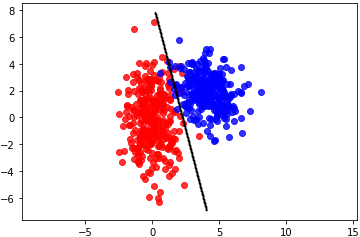
\includegraphics[width=.8\linewidth]{Code/images/42/LDAex}
		\caption{LDA}
	\end{subfigure}%
	\begin{subfigure}{.5\textwidth}
		\centering
		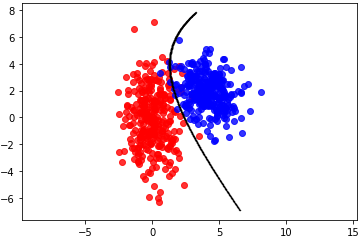
\includegraphics[width=.8\linewidth]{Code/images/42/QDAex}
		\caption{QDA}
	\end{subfigure}
	\caption{Example of LDA and QDA where the decision boundary is shown in black.}
	\label{fig:LQDAex}
\end{figure}
We note that both LDA and QDA are equivalent to the Bayes rule \ref{bayesclass} when the assumptions of normality and homoscedasticity (for the LDA) are satisfied. Indeed, the likelihood ratio $f_1(x)/f_0(x)$ is equal to the Radon-Nikodym derivative of the two induced Gaussian measures in this case. Thus, under these assumptions, LDA and QDA are optimal classifiers.

In practice, none of the parameters $\mu_i,\Sigma_i$ are known. They can be estimated in the usual way by the empirical estimators $\hat{\mu}_i,\hat{\Sigma}_i$. These can then be plugged into either the LDA or QDA rules. Since these estimators converge to their associated real values, LDA and QDA using these estimates are asymptotically optimal.

Without the Gaussian assumption, LDA can still be seen as the optimal linear classifier in the following sense. Suppose here that $p=1/2$, then the direction $v$ with $\Vert v\Vert=1$ maximizing the variance of $v^TX$ is $w$ given by the LDA rule, where $X\sim \frac{1}{2}\Pi_0 + \frac{1}{2}\Pi_1$. Indeed, we have 
\begin{eqnarray*}
	\mathrm{Var}[v^T X] & = & \E[\mathrm{Var}[v^TX\mid \Pi]] + \mathrm{Var}[\E[v^TX \mid \Pi]] = v^T\Sigma v + \left(v^T\left(\frac{\mu_0-\mu_1}{2}\right)\right)^2 \\
	& = & v^T \left(\Sigma + \left(\frac{\mu_0-\mu_1}{2}\right)\left(\frac{\mu_0-\mu_1}{2}\right)^T \right)v\\
	& = & (\Sigma^{1/2} v)^T \left(I + \Sigma^{-1/2}\left(\frac{\mu_0-\mu_1}{2}\right)\left(\frac{\mu_0-\mu_1}{2}\right)^T\Sigma^{-1/2} \right)(\Sigma^{1/2} v)
\end{eqnarray*}
The maximum of this last expression, conditioned on $\Vert v\Vert=1$, is attained when $\Sigma^{1/2}v$ is the first eigenvector of the matrix in the middle. This eigenvector is easily seen to be $\Sigma^{-1/2}(\frac{\mu_0-\mu_1}{2})$, giving
$$v = \Sigma^{-1}\left(\frac{\mu_0-\mu_1}{2}\right) \propto w.$$
Intuitively, the direction maximizing $\mathrm{Var}[v^T X]$ is the one on which the projections of the two populations are the most well-separated.

\subsection{Infinite dimensional case: Equivalent Gaussian measures}
In the infinite dimensional case, densities do not exist (as there is no Lebesgue measure, see Prop. \ref{noleb}). However, for separable Hilbert spaces and Gaussian random element on them, the theory developed in the last chapter allows us to construct powerful classifiers. \\
For example, suppose we have to populations on a separable Hilbert space $H$, $\Pi_0,\Pi_1$, that follow have Gaussian distributions with mean $\mu_0,\mu_1$ and same covariance operator $Q$. Suppose further that $\mu_1-\mu_0 \in Q^{1/2}(H)$. Then, using Theorem \ref{radnikgauss}, one can construct the Bayes classifier $\mathbf{1}[C^*(x)>1]$ with (assume $p=1/2$)
$$C^*(x) = \frac{dN_{\mu_1,Q}}{dN_{\mu_0,Q}}(x) =  \exp\left[\langle Q^{-1/2}(\mu_1-\mu_0),Q^{-1/2}(x-\mu_0)\rangle - \frac{1}{2} \Vert Q^{-1/2}(\mu_1-\mu_0)\Vert^2 \right].$$
Equivalently, it classifies to $\Pi_1$ if 
\begin{eqnarray*}
	& & \frac{1}{2} \Vert Q^{-1/2}(\mu_1-\mu_0)\Vert^2 <\langle Q^{-1/2}(\mu_1-\mu_0),Q^{-1/2}(x-\mu_0)\rangle  \\
	& \iff & \frac{1}{2} \Vert Q^{-1/2}(\mu_1-\mu_0)\Vert^2 + \langle Q^{-1}(\mu_1-\mu_0),\mu_0\rangle < \langle Q^{-1}(\mu_1-\mu_0),x\rangle.
\end{eqnarray*}
This rule is, mutatis mutandis, the same as the LDA rule in finite dimension. We therefore also call it the LDA rule. As in finite dimension, the classification depends only on the projection of $x$ on the 1-dimensional subspace spanned by $Q^{-1}(\mu_1-\mu_0)$. Therefore, the LDA rule reduces the classification of infinite dimensional objects, like functions, to a one dimensional problem.\\
As in the finite dimensional case, such a nice linear behavior is not present when the covariance operator of the two populations is not the same. In that case, one can in general still write down the Radon-Nikodym derivative, see \cite[Coro. 6.4.11]{boga}, and thus use the Bayes classifier as above. This yields a generalization of the QDA rule. See also Section \ref{qdainf} for a more direct approach.  \\
The proof that LDA is the variance-maximizer linear classifier is still valid in the Hilbert space framework. One needs just one the inner product in $H$ instead of that of $\R^d$. The LDA rule is also optimal in another way: it is the best linear centroid classifier, see \cite[Section 2.2]{DH3}. A centroid classifier classifies a sample $x$ to population $\Pi_1$ if and only if $d(x,\mu_1)<d(x,\mu_0)$,
where $d$ is a (pseudo)metric on $H$. When the distance used is 
$$d_v(x,\mu_i) = \vert \langle x,v \rangle - \langle \mu_i, v\rangle\vert,$$
we call it the linear centroid classifier with direction $v$. One easily sees that the LDA rule is equivalent to 
$$0 < d_v^2(x,\mu_0)-d_v^2(x,\mu_1),$$
with $v=Q^{-1}(\mu_1-\mu_0)$. Thus, it is a linear centroid classifier. The next proposition shows that it is optimal. 
\begin{prop}
	Let $\Pi_0,\Pi_1$ have a Gaussian distribution with mean $\mu_0,\mu_1$ and covariance $Q$. Suppose $\mu_1-\mu_0 \in Q^{1/2}(H)$. Then, the linear centroid classifier having the lowest misclassification probability is the one with direction $Q^{-1}(\mu_1-\mu_0)$.
	\begin{proof}
		Lets compute the probability of misclassifying an element from population $\Pi_1$ in population $\Pi_0$:
		\begin{eqnarray*}
			\Pp_{\Pi_1}\left[d_v(x,\mu_1)\geq d_v(x,\mu_0)\right] & = & \Pp_{\Pi_1}\left[\left(\langle x,v\rangle- \langle \mu_1,v\rangle\right)^2\geq \left(\langle x,v\rangle- \langle \mu_0,v\rangle\right)^2\right] \\
			& = & \Pp_{\Pi_1}\left[2\langle x,v \rangle\langle \mu_0-\mu_1,v \rangle + \langle \mu_1,v \rangle^2 - \langle \mu_0,v \rangle^2 \geq 0 \right] \\
			& = & \Pp_{\Pi_1}\left[ \langle x, v \rangle \geq \frac{\langle \mu_0 + \mu_1, v \rangle}{2}  \right] = 1 - \Phi\left(\frac{\langle\mu_0-\mu_1,v\rangle}{2\sqrt{\langle Qv,v\rangle}}\right)
		\end{eqnarray*}
		A quick computation shows that $\Pp_{\Pi_1}\left[d_v(x,\mu_1)\geq d_v(x,\mu_0)\right] = \Pp_{\Pi_0}\left[d_v(x,\mu_1) < d_v(x,\mu_0)\right]$, so that the overall probability of misclassification is 
		\begin{equation}\label{probmisclass}
			\frac{1}{2}  \Pp_{\Pi_1}\left[d_v(x,\mu_1)\geq d_v(x,\mu_0)\right] + \frac{1}{2}\Pp_{\Pi_0}\left[d_v(x,\mu_1) < d_v(x,\mu_0)\right] = 1 - \Phi\left(\frac{\langle\mu_0-\mu_1,v\rangle}{2\sqrt{\langle Qv,v\rangle}}\right).
		\end{equation}
		The problem of minimizing the misclassification probability is thus equivalent to the maximization problem
		$$ \max_{v\in H} \frac{\langle\mu_0-\mu_1,v\rangle}{\sqrt{\langle Qv,v\rangle}} \iff \max_{v\in H} \frac{\langle\mu_0-\mu_1,v\rangle^2}{\langle Qv,v\rangle}.$$
		Now, by the Cauchy-Schwarz inequality, 
		$$ \frac{\langle\mu_0-\mu_1,v\rangle^2}{\langle Qv,v\rangle} = \frac{\langle Q^{-1/2}(\mu_0-\mu_1),Q^{1/2}v\rangle^2}{\langle Q^{1/2}v,Q^{1/2}v\rangle} \leq \frac{\Vert Q^{-1/2}(\mu_0-\mu_1)\Vert^2 \ \Vert Q^{1/2}v\Vert^2 }{\Vert Q^{1/2}v\Vert^2} = \Vert Q^{-1/2}(\mu_0-\mu_1)\Vert^2,$$
		where the inequality is an equality if and only if 
		$$ v \propto Q^{-1}(\mu_0-\mu_1).$$
		In particular, the LDA direction $v=Q^{-1}(\mu_1-\mu_0)$ achieves this maximum and is thus optimal.
	\end{proof}
\end{prop}
The proof of the previous proposition shows that the misclassification probability of LDA is $1-\Phi\left(\Vert Q^{-1/2}(\mu_1-\mu_0)\Vert/2\right)$. Thus, the larger $\mu_1-\mu_0$ is in the RKHS of $Q$, the better the classification is.\\
We note that although the analysis of these classifiers is performed with the assumptions that the distributions are Gaussian, they also perform well when this assumption is not satisfied. 
\subsection{Infinite dimensional case: Singular Gaussian measures}
A natural question now is: what happens when $\mu_1-\mu_0 \notin Q^{1/2}(H)$? In that case, by Theorem \ref{radnikgauss}, the distributions of $\Pi_0$ and $\Pi_1$ are singular. Let $A,B\in \mathcal{B}(H)$ form a partition of $H$ with $N_{\mu_0,Q}(B)=N_{\mu_1,Q}(A)=0$. Then, a perfect classifier would be $\mathbf{1}[x\in B]$, see Section \ref{sec:introclass}. The sets $A$ and $B$ cannot be written down explicitly. However, using the LDA approach, one can construct sequences of classifiers $C_n(x)$ that are asymptotically perfect, i.e.,
$$\lim_{n\to \infty} \left(\frac{1}{2}\Pp_{\Pi_0}[C_n(x)=1] + \frac{1}{2}\Pp_{\Pi_1}[C_n(x)=0]\right)=0.$$
Following \cite{Kraus2}, we will present three techniques for constructing such sequences based on the LDA classifier.

The first one is just to project the problem on the first few principal components of the data. More precisely, let $\{\lambda_i,\phi_i\}_{i=1}^\infty$ be a complete orthonormal system of eigenvectors of $Q$. Then, since $\mu_1-\mu_0 \notin Q^{1/2}(H)$, we must have 
\begin{equation}\label{serinftylol}
	\sum_{i=1}^{\infty} \frac{\langle \mu_1 -\mu_0, \phi_i\rangle^2 }{\lambda_i} = \infty.
\end{equation}
The LDA direction $w = Q^{-1}(\mu_1-\mu_0)$ does not belong to $H$. However, one can `approximate' it in the subspace spanned by the first $m$ principal components $\{\phi_i\}_{i=1}^m$:
$$w_m = \sum_{i=1}^{m} \frac{\langle \mu_1 -\mu_0, \phi_i\rangle }{\lambda_i}\phi_i.$$
By Equation \ref{probmisclass}, the misclassification probability of the linear centroid classifier with direction $w_m$ is given by $1-\Phi(\Upsilon_m)$ with 
\begin{equation*}
	\Upsilon_m =  \frac{\langle \mu_1 - \mu_0, w_m\rangle }{2\sqrt{\langle Qw_m,w_m\rangle}} = \frac{\langle \mu_1-\mu_0, w_m\rangle}{2\Vert Q^{1/2}w_m \Vert},
\end{equation*}
and 
$$ Q^{1/2}w_m = \sum_{i=1}^\infty \sqrt{\lambda_i} \langle w_m,\phi_i\rangle \phi_i = \sum_{i=1}^{m} \frac{\langle \mu_1 -\mu_0, \phi_i\rangle }{\sqrt{\lambda_i}}\phi_i, \ \Vert Q^{1/2}w_m \Vert^2 = \sum_{i=1}^{m} \frac{\langle \mu_1 -\mu_0, \phi_i\rangle^2 }{\lambda_i} $$
so that 
$$\Upsilon_m = \frac{1}{2} \Vert Q^{1/2}w_m\Vert \stackrel{m \to \infty}{\longrightarrow} \infty \ \text{ (by Equation \ref{serinftylol}).}  $$ 
Therefore, the misclassification probability of the linear centroid classifier with direction $w_m$  goes to 0 as $m$ goes to infinity. This sequence of classifiers is thus asymptotically perfect.

The sequence of directions $w_m$ above is gotten by projecting the LDA direction on the subspaces $\mathrm{span}\{\phi_1,...,\phi_m\}$. We note that these subspaces do not depend on $\mu_0$ nor $\mu_1$. It should therefore be expected that there exist better sequences of subspaces on which one can project the LDA direction. One such sequence is the sequence of Krylov subspaces 
$$K_m = \mathrm{span}\left\{\mu_1-\mu_0,...,Q^{m-1}(\mu_1-\mu_0)\right\}.$$
Projecting an element on these subspaces yields the conjugate gradient algorithm presented in \cite[Algo.\! 1]{Kraus2}. These subspaces depend on $\mu_0$ and $\mu_1$ and the next proposition shows that they give better classifiers than the principal component subspaces. 
\begin{prop}\cite[Prop.\! 2]{Kraus2}
	For any $m$, projecting the LDA solution on $K_m$ gives a smaller misclassification probability than projecting it on the first $m$ principal components.
\end{prop}
In particular, it is asymptotically perfect.

Finally, the third approach is to project the LDA direction on balls of finite radii. This is done by using the directions 
$$w_\alpha = (Q + \alpha I)^{-1}(\mu_1-\mu_0) \ \text{ with } \alpha\to 0_+.$$  
This last expression makes sense:
$$\sum_{i=1}^{\infty} \frac{\langle \mu_1 -\mu_0, \phi_i\rangle^2 }{(\lambda_i + \alpha)^2} = \frac{1}{\alpha^2} \sum_{i=1}^{\infty} \frac{\langle \mu_1 -\mu_0, \phi_i\rangle^2 }{(\lambda_i/\alpha + 1)^2} \leq \frac{1}{\alpha^2} \sum_{i=1}^{\infty} \langle \mu_1 -\mu_0, \phi_i\rangle^2 = \frac{1}{\alpha^2}\Vert \mu_1-\mu_0 \Vert^2 < \infty.$$
The  misclassification probability is given by $1-\Phi(\Upsilon_\alpha)$ with
\begin{equation*}
	\Upsilon_\alpha  =  \frac{\langle\mu_0-\mu_1,w_\alpha\rangle}{2\sqrt{\langle Qw_\alpha,w_\alpha\rangle}}.
\end{equation*}
Using 
$$\sum_{i=1}^{\infty} \frac{\lambda_i \langle \mu_1 -\mu_0, \phi_i\rangle^2}{(\lambda_i + \alpha)^2} \leq \sum_{i=1}^{\infty} \frac{(\lambda_i+\alpha) \langle \mu_1 -\mu_0, \phi_i\rangle^2}{(\lambda_i + \alpha)^2} = \sum_{i=1}^{\infty} \frac{\langle \mu_1 -\mu_0, \phi_i\rangle^2}{\lambda_i + \alpha},$$
we get 
$$\Upsilon_\alpha = \frac{\sum_{i=1}^{\infty} \frac{\langle \mu_1 -\mu_0, \phi_i\rangle^2}{\lambda_i + \alpha}}{\left(\sum_{i=1}^{\infty} \frac{\lambda_i \langle \mu_1 -\mu_0, \phi_i\rangle^2}{(\lambda_i + \alpha)^2}\right)^{1/2}} \geq \left( \sum_{i=1}^{\infty} \frac{\langle \mu_1 -\mu_0, \phi_i\rangle^2}{\lambda_i + \alpha} \right)^{1/2} \stackrel{\alpha\to 0_+}{\longrightarrow} \infty \text{ by Equation \ref{serinftylol}.}$$
Therefore, using $\alpha = 1/m$, we get a sequence of classifiers that is asymptotically perfect.

All three methods presented above work in the same way. They project the LDA direction on various sequences of subsets of $H$: the principal component subspaces, the Krylov subspaces or balls of increasing radii. These give sensible approximation of the non-existing $Q^{-1}(\mu_1-\mu_0)$. However, when the latter does exist, it still makes sense to use these methods and see them as regularization techniques. As all three sequences converge to the range of $Q$, it is easy to prove that the induced sequences of direction $w_m$ converge to the LDA direction $Q^{-1}(\mu_1-\mu_0)$ when it exists.

\subsection{QDA for infinite dimensional data}\label{qdainf}
Consider now the classification framework where two populations $\Pi_0$ and $\Pi_1$ have means $\mu_0$ and $\mu_1$ and covariance operators $Q_0$ and $Q_1$. Then, we can adapt the QDA rule \ref{qdarule} in this setting. This cannot be done directly, since the determinant of an operator is not well-defined and since the inverses $Q_0^{-1},Q_1^{-1}$ do not exist in general. However, one can get around these issues by truncating these operations at order $m$. More precisely, let $\{\lambda_i,\phi_i\}_{i=1}^\infty$ and $\{\nu_i, \psi_i\}_{i=1}^\infty$ be complete orthonormal system of eigenvectors of $Q_0$ and $Q_1$ respectively. Then, one can use the following approximations 
$$\log \vert Q_0\vert \rightsquigarrow \sum_{i=1}^{m} \log \lambda_i \ \ \text{ and } \ \ Q_0^{-1} \rightsquigarrow \sum_{i=1}^{m} \frac{1}{\lambda_i} \phi_i \otimes \phi_i,$$
and similarly for $Q_1$. These yield the following QDA classifier: we classify an observation $x$ to population $\Pi_1$ if and only if
$$2\log\left(\frac{p}{1-p}\right) < \sum_{i=1}^{m} \left[\log\left(\frac{\lambda_i}{\nu_i}\right) + \frac{\langle x-\mu_0,\phi_i\rangle^2 }{\lambda_i} - \frac{\langle x-\mu_1,\psi_i\rangle^2 }{\nu_i}\right].$$ 
In \cite[Theorem 1]{DH1}, it is shown that under various conditions, this classifier is asymptotically perfect as $m$ goes to infinity. We are, however, still looking for a clean proof that this classifier is asymptotically perfect when the distributions of $\Pi_0$ and $\Pi_1$ are singular.

\section{Classification of functional fragments}
We now investigate the problem of classifying functional fragments. We use the same framework and notations as in Chapter \ref{chap:frags}. We will work in the following classification framework: we assume $H=\Ll^2[0,1]$, there are two populations $\Pi_0$ and $\Pi_1$ on $H$ and a probability distribution $\upsilon$ on the set of subintervals of $[0,1]$ that is independent of $\Pi_0$ and $\Pi_1$. Given a new observation $(X,[a,b])$, we want to decide whether $X$ comes from population $\Pi_0$ or $\Pi_1$.\\
In that form, this framework is (intentionally) too vague. For example, here are some possibilities:
\begin{enumerate}
	\item We have full information on the distribution of $\Pi_0$ and $\Pi_1$ and need to classify fragments.
	\item We observe fragments and need to classify fragments.
	\item We observe fragments and need to classify full curves.
	\item We observe full curves and need to classify fragments.
\end{enumerate}
To the best of our knowledge, only two papers have been written exclusively on that subject in the FDA literature, \cite{DH1} and \cite{Kraus2}. We will next present the methods given in these papers. We also note that in the case where the functions are observed only on a finite grid, which is always the case in practice, methods from machine learning, in particular the use of recurrent neural networks, have been developed to solve these classification tasks. 

First, we describe a general approach to the classification of functional fragments. The ``training'' procedure yields information on the populations $\Pi_0$ and $\Pi_1$, typically in the form of estimates of the means $\hat{\mu}_0,\hat{\mu}_1$ and covariance kernels $\hat{K}_0,\hat{K}_1$ of $\Pi_0$ and $\Pi_1$. We can also assume homoscedasticity and have an estimate $\hat{K}$ of the common covariance kernel. It can also be, as in case 1. above, that the true values of these parameters are given. Then, given a new observation $(X,[a,b])$, we use the functional classification techniques, e.g. LDA and QDA, on this observation by restricting the problem to $[a,b]$. For example, we use LDA on $X\in \Ll^2[a,b]$ with parameters
$$\hat{\mu}_0\!\mid_{[a,b]}, \ \hat{\mu}_1\!\mid_{[a,b]} \ \text{and} \ \hat{K}\!\mid_{[a,b]\times[a,b]}.$$
This gives a general method for the classification of functional fragments. We will see next how one can estimate $\hat{\mu}_j$, $\hat{K}_j$ in clever ways to achieve better classification accuracy.

In \cite{DH1}, the authors use their curve extension method, described in Section \ref{sec:curveext}, to get more information on the population $\Pi_0$ and $\Pi_1$ and to then achieve a better classification accuracy. More precisely, it is assumed that fragments 
$$(X_{0,1},\Oo_{0,1}),...,(X_{0,n_0},\Oo_{0,n_0})\stackrel{i.i.d}{\sim} \Pi_0 \otimes \upsilon \ \text{ and } \ (X_{1,1},\Oo_{1,1}),...,(X_{1,n_1},\Oo_{1,n_1})\stackrel{i.i.d}{\sim} \Pi_1 \otimes \upsilon$$
are observed. Then, a new observation $(X,[a,b])$ is classified in the following way: the observed fragments are all extended to $\tilde{X}_{j,i}$ on an interval
$$\I \supset \bigcup_{i=1}^{n_0}\Oo_{0,i} \ \cup \ \bigcup_{i=1}^{n_1}\Oo_{1,i} \ \cup \ [a,b]$$
using the gluing method. Weights $w_{j,i}$ quantifying how far the interval $\Oo_{j,k}$ is from the interval $\I$ are computed for $j=0,1$, $i=1,...,n_j$. The means and covariance kernels of both populations are are computed by
$$\hat{\mu}_j(t) = \frac{1}{n_j} \sum_{i=1}^{n_j} w_{j,i}\tilde{X}_{j,i}(t) \ \text{ and } \ \hat{K}_j(s,t) = \frac{1}{n_j} \sum_{i=1}^{n_j} w_{j,i}\left[(\tilde{X}_{j,i}(s)-\hat{\mu}_j(s))(\tilde{X}_{j,i}(t)-\hat{\mu}_j(t))\right],$$
for $j=0,1$, $s,t \in \I$. Finally, the curve $X$ on $\I$ is classified using the QDA method described in Section \ref{qdainf}. The LDA rule can also be used if all the observations are aggregated when estimating the covariance kernel. In \cite[Section 5.2]{DH1}, it is shown that under some conditions this classifier performs better than using QDA (or LDA) without curve extensions. 

In \cite{Kraus2}, the framework is the same as above. Their approach to the classification of fragments is, however, more pragmatic. They consider the smallest common domain of all curves
$$\I_0 = \bigcap_{i=1}^{n_0}\Oo_{0,i} \ \cap \ \bigcap_{i=1}^{n_1}\Oo_{1,i} \ \cap \ [a,b]$$
and the largest subdomain $\I^{max}$ of $[a,b]$ where enough curves have been observed. They then consider a chain of domains
$$\I_0 \subset \I_1 \subset ... \subset \I_K = \I^{max} \subseteq [a,b].$$
For all such subdomains $\I_j$, the estimated means $\hat{\mu}_0^j,\hat{\mu}_1^j$ and common covariance $\hat{K}^j$ are computed using the naive estimators given in Section \ref{naiveest}. They then perform cross-validation on all the $\I_j$'s to estimate the misclassification rate on each using LDA with one of the regularization techniques presented in the last section. Finally, they classify the observation $(X,[a,b])$ on the subdomain having the lowest cross-validation misclassification rate. The idea behind this approach is that performing classification only on $\I_0$ might be too restrictive since a big fraction of the curves will be ignored. On the other hand, using $\I^{max}$ might be too optimistic since many curves may be unobserved on this domain and so the estimations of the means and covariance may be too biased. Thus, this algorithm looks for the right balance between these two extreme subdomains.\\
We note that this approach is designed for when the fragments are observed in the ``blanket'' regime (see Section \ref{introfrag}). Indeed, in that regime the smallest common domain $\I_0$ is already quite large and so classification can be performed meaningfully on it. In the ``banded'' regime, $\I_0$ is typically small, even empty when $\delta<0.5$. 

Finally, we present a novel approach based on the covariance recovery of \cite{DP2}. We use the same framework as above and assume further that we are in the ``banded'' regime, i.e., that all observations are of length $\delta \in (0,1)$. The naive estimates of the means $\hat{\mu}_0,\hat{\mu}_1$ and covariance kernels $\tilde{K}_0,\tilde{K}_1$ are computed. As before, we can also assume homoscedasticity and get an estimate $\tilde{K}$ of the common covariance kernel. Then, using the matrix completion method, we get estimates $\hat{K}_0,\hat{K}_1$ of rank $r_0,r_1$. Finally, a new observation $(X,[a,b])$ is classified using QDA with parameters 
$$\hat{\mu}_0\!\mid_{[a,b]}, \ \hat{\mu}_1\!\mid_{[a,b]}, \  \hat{K}_0\!\mid_{[a,b]\times[a,b]} \ \text{and} \ \hat{K}_1\!\mid_{[a,b]\times[a,b]},$$
or LDA with $\hat{K}\!\mid_{[a,b]\times[a,b]}$. In the case where $b-a\leq \delta$, this can be seen as a regularization technique on the covariance kernel estimation by intentionally reducing the rank of the naive estimates. In the case where $b-a>\delta$, the matrix completion method recovers new meaningful information on the kernels outside of the band $\{|s-t| \leq \delta\}$. This can be used to classify longer fragments with more accuracy.


\section{A probabilistic approach to classification}
\subsection{Explain the perfect classification phenomenon through the F-H theorem. If I manage to find something, also the classification of fragments.}

\chapter{Numerical experiments}









\bibliography{biblio} 
\bibliographystyle{hapalike}



\end{document}